\documentclass[12pt]{article}
\usepackage{graphicx}
\usepackage{graphics}
\usepackage[percent]{overpic}
\usepackage{hyperref}
\usepackage{indentfirst}
%\usepackage{setspace}
\renewcommand\theequation{{\color{red}\arabic{equation}}}
\hypersetup{colorlinks=true}
\usepackage{amsmath}
\usepackage{empheq}
\usepackage{amsfonts,amssymb}
\usepackage{float}
\usepackage{algorithm}
\usepackage{algorithmic} 
\usepackage{caption}
\usepackage{subfigure}
%\usepackage{subcaption}
\usepackage[numbers]{natbib}
\usepackage{lipsum}
\bibliographystyle{abbrvnat}%{ieeetr}%Choose a bibliograhpic style
\usepackage[toc,page]{appendix}
\addtolength{\textwidth}{1.1in}
\addtolength{\hoffset}{-0.5in}
\addtolength{\textheight}{1.1in}
\addtolength{\voffset}{-0.8in}
\usepackage{tikz,pgfplots}
\usetikzlibrary{arrows,snakes,backgrounds,spy,mindmap,trees}
\usetikzlibrary{er}
%\usepackage{onimage}
\pgfplotsset{compat=newest}
%\usepackage{setspace}
%\doublespacing
%\usepackage{parskip}
%\parskip=2\baselineskip \advance\parskip by 0pt plus 2pt 
\usepackage{rotating}
\newcommand{\mgnote}[1]{\textcolor{magenta}{MG: #1}}
\newcommand{\gsnote}[1]{\textcolor{blue}{GS: #1}}
\newcommand{\vrnote}[1]{\textcolor{red}{VR: #1}}
\newcommand{\IIinv}{{\dot\varepsilon}_{\mathrm{\!\!\:II}}}
 
\newcommand{\mm}{{\ensuremath{\boldsymbol{m}}}}
\newcommand{\uu}{{\ensuremath{\boldsymbol{u}}}}
\newcommand{\vv}{{\ensuremath{\boldsymbol{v}}}}
\newcommand{\ww}{{\ensuremath{\boldsymbol{w}}}}
\newcommand{\uobs}{{\ensuremath{\boldsymbol{u}_\text{obs}}}}
\newcommand{\ff}{{\ensuremath{\boldsymbol{f}}}}
\newcommand{\FF}{{\ensuremath{\boldsymbol{F}}}}
\newcommand{\ppi}{{\ensuremath{\boldsymbol{\pi}}}}

\newcommand{\ssigma}{{\ensuremath{\boldsymbol{\sigma}}}}
\newcommand{\strain}{{\ensuremath{\dot{\boldsymbol{\varepsilon}}}}}


%\let\oldabstract\abstract
%\let\oldendabstract\endabstract
%\makeatletter
%\renewenvironment{abstract}
%{\renewenvironment{quotation}%
%               {\list{}{\addtolength{\leftmargin}{1em} % change this value to add or remove length to the the default
%                        \listparindent 1.5em%
%                        \itemindent    \listparindent%
%                        \rightmargin   \leftmargin%
%                        \parsep        \z@ \@plus\p@}%
%                \item\relax}%
%               {\endlist}%
%\oldabstract}
%{\oldendabstract}
%\makeatother




\date{}

\title{Chapter 4: Simultaneous inference of plate boundary properties and mantle viscosity with an adjoint optimization: Large scale two-dimensional models}


\begin{document}
\maketitle
\begin{abstract}
 Plate motions are a primary surface constraint on forward models of plate and mantle dynamics, rheology, plate boundary stresses, and models for the occurrence of great earthquakes. Estimates of effective viscosity regionally (from post-glacial rebound and post seismic relaxation) provide additional constraints on mantle dynamics. 
Here we incorporate plate motion and effective viscosity data into an optimization and derive an adjoint, gradients for inferred parameters, and posterior distributions for  rheological paramters, stresses within plate boundaries, and the effective viscosity of subducted slabs. 
We apply these methods to 2-D cross-sections of subduction zones, with temperature distributions and fault zone geometries developed from seismic and other data. 
Analyzing the conditional and marginal distributions, we find that the 
Tonga and the Marianas subduction zones have the lowest values of mechanical coupling while Chile and Sumatra the highest, among those studied. The subduction zones with the lowest coupling have back-arc extension. Globally, we find that the non-linear stress-strain exponent, $n$, is 3.0 $\pm$ 0.25 (in the upper mantle and lithosphere) with a pressure-independent yield stress of 150 $\pm$ 25 MPa. The stress in shear zones is tens of MPa and the shear and the normal stresses are elevated in seismically coupled compared to uncoupled subduction zones. 
Relative differences in inferred mechanical couplings are similar to observed seismic coupling. 
We find that within the hinge zone for Sumatra and Nazca-South America subduction zones, the average effective viscosity is on the order of $10^{21} Pa\cdot s$, while the least seismically coupled (Tonga, Ryukyu and Izu-Bonin) have an average effective viscosity on the order of $10^{22} Pa\cdot s$. This partition of average effective viscosity suggests that there is a link between plate coupling and the average dynamic weakening for seismically coupled subduction zones.
\end{abstract} 


\section{Introduction}

\mgnote{Can you start using the formatiing for the referencing eith in the Caltech Thesis or GJI Style?}

While slab pull may be the dominant force driving plate motions and associated mantle flow, there remains uncertainty on the relative coupling of stresses across plate boundaries at subduction zones. This coupling can either be attributed to broad-scale tectonic forces or the varying properties between plates at each subduction zone. While it is not clear whether broad-scale forces or the varying properties have the stronger contribution to the variations in seismic coupling, a valid model should appropriately represent the broad-scale forces. 
Seismic coupling is defined as the ratio between the observed seismic moment release to the rate of plate tectonic velocities and generally varies between 0 and 1 \citep{davies1971regional}. 
Seismic coupling is sensitive to the short window of recorded earthquakes such that if many large magnitude earthquakes occur within that short window 
at a greater rate than the long-term average, then the seismic coupling could be close to or even exceed unity, whereas if the earthquakes occur at an unusally low rate, inferred seismic coupling will be small.  While seismic coupling is a reasonable way to build a relationship to forecast which subduction zones have a propensity for future large events, additional data, for example, the curvature of subduction zones \citep{bletery2016mega} or along-strike gravity anomalies \citep{song2003large}, 
can better condition such forecasts. 

  %It was suggested in \citep{ide2013proportionality} that background seismicity can be correlated with subduction zones that have experienced great earthquakes. %Additionally, there might be a correlation between the plate age and b-value \citep{nishikawa2014earthquake}. These results lead to relating the shear and normal stresses (broad-scale forces) at plate boundaries to background seismicity and b-values in addition to the geodetic seismic coupling.

Regardless of whether broad-scale forces or varying shear zone properties are the ultimate cause for variations in seismic coupling, geodynamic models should be able to explain variations between the two end-members from the least coupled Marianas to the coupled Chilean subduction zone. 
The Chilean subduction zone is among the most seismically active with many earthquakes above 8, including the 1960 Valdivia earthquake with moment magnitude 9.5 \citep{kanamori1974},
the largest ever recorded. 
On the other hand the Marianas subduction zone is among the least seismically coupled with no historic earthquakes greater than magnitude 7.7 \citep{mccaffrey2008global}. 
Chile, overall is in a state of compression on the South American margin, while, the Marianas subduction zone is characterized by active back arc opening indicative of regional tension.


A simple force balance of subduction that parameterizes the broad-scale forces suggests a link between tectonic forces and the degree of seismic coupling \citep{scholz1995mechanism, scholz2012seismic}. 
These models estimate the force distribution that arises from slab pull and a putative anchoring force, for each subduction zone. Such models do not include key variations in rheology and how such variations would influence the distribution of  normal forces.  While the analysis found a relationship between broad-scale forces and coupling, their approach may not capture the essence of the system as the actual geometry of slabs is complex with substantial variations induced by global flow \citep{scholz2012seismic}. 
Although simple, these force balance models haven't found general acceptance.

%The partitioning of the resisting forces can be seen through the plate-coupling of the weakzone factors in the rheological relationship, which provides the effective frictional resistance in models. There have been investigations into these ideas and how different subduction zones have different fricitional forces.  The notion of coupling can be either mechanical or tectonic coupling. Both ideas can lead to the end member cases 

  To accurately estimate the forces at plate boundaries, not only is the correct physics needed, but an optimization scheme must be constrained by observed plate motions \citep{BursteddeStadlerAlisicEtAl13,Stadler27082010}, the most robust constraint on mantle flow. We overcome these limitations by employing an approach  similar to that introduced earlier \citep{ratnaswamy2015adjoint}, with plate motion data used for areas away from deforming plate boundaries, essentially allowing for self-consistent deformation within plate boundaries. 
Furthermore, the shape of fault zones play a key role in governing plate motions \citep{Zhong10021995}, and these can be mapped at shallow depths with seismic observations and are needed as constraints.
Augmenting surface velocities, we now incorporate constraints on the average viscosity within selected regions. Estimates of the average effective viscosity arise from post-glacial rebound and post-seismic relaxation. Using constraints on viscosity may allow for a better estimation of the strain rate exponent, upper mantle prefactor and bulk effective mantle properties compared to an optimization that solely uses plate motion data. 
The viscosity reduction for a shear zone representing the megathrust between plates has been inferred from the adjoint-based optimization, but not the state of stress. We show that such stresses can be estimated from an additional adjoint solve.
We determine the trade-offs between the calculated stresses and inferred rheological parameters. 





In this chapter, we will explore the incorporation of average effective viscosities and estimation of stress uncertainty in fault zones. While inferring plate boundary strength factors \citep{ratnaswamy2015adjoint} can lead to a better understanding of which plate boundaries are more mechanically coupled, \mgnote{This needs to be stated much more precisely. I don't think that it is their non-dimensionalization which is at issue. I beleive that it is a difference between an intrinsice versus extrinsic properties. I think stress is extrinsice while rheological parameters are intrinsic. Georg what do you think about this comment?} such variables are non-dimensional and so here we not only estimate the magnitude of  stresses but also their uncertainties. We will derive expressions for the gradients of inferred parameters using average effective viscosity and expressions for the covariance matrices of the average normal and shear stresses. We then apply these methods to 2D cross-sectional slices with observed plate motions and viscosity constraints and thermal structures and fault zone geometries constrained by a variety of other (but primarily seismic) data.

Models with a simple parameterization of plate boundary strength, 
in which no mechanical distinction is made between the bending plate and the
zone of inter-plate coupling are to be avoided.
Plate bending and interplate coupling are observationally
resolved and distinct processes and if we hope to understand the
plate tectonic controls on interplate seismic coupling
and how slab strength may influrnce plate motions, while moving forward
with a new framework to link geodynamics to the occurance of great
earthquakes, then the more complete
formulation we have adopted is essential.
 
\section{Forward Model}

The underlying physics of mantle flow is governed by the creeping of mantle rocks under geological time scales. 
Over time scales greater than about 1 year result the deformation of the mantle behaves as a viscous fluid governed by the Stokes equations
\begin{equation}
  \label{eq:stokes}
  \begin{split}
    \nabla \cdot \uu &=0 \qquad  \text{on } \Omega, \\
    \nabla \cdot \ssigma&=-\text{Ra}T \textbf{e}_r  \qquad \text{on } \Omega, \\
  \end{split}
\end{equation}
with free slip boundary conditions
\begin{align*}
  \uu\cdot \textbf{n}&=0 \quad \text{on} \, \partial \Omega, \\
 \boldsymbol{\mathrm{T}}(\ssigma \textbf{n})
  &= \:0 & \text{ on }\partial \Omega
  \label{eq:bc}
\end{align*}
with viscous stress tensor being  $\ssigma := 2\eta(T,n,\ssigma_y)-p\textbf{I}$ where $p$ is the forward pressure, and \mgnote{Use a different font for Tangential operator that is distinct from temperature and the Transpose}\vrnote{done}{$\boldmath{\mathrm{T}}$ is the tangential operator ($\boldmath{\mathrm{T}} = \textbf{I} - \textbf{n} \otimes \textbf{n}$). Furthermore, the momentum equation in ~\eqref{eq:stokes} is driven by thermal buoyancy where \textit{T} is the temperature field and \textit{Ra} is the thermal Rayleigh number. Solving the Stokes equations, we obtain the solution of the forward velocities ($\uu$) and pressures ($p$). An important part of the stress tensor $\ssigma$ is the rheological relationship. In our forward model we use a nonlinear rheology where we take into account the shear-thinning nature of the upper mantle through the use of a power law rheology with a strain rate exponent
and the diffusion creep in the lower mantle with a linear rheology, while using a global yield stress to allow for dynamic weakening (which primarily occurs within the hinge zones, that is where slabs bend). 
Our viscosity formulation is 
\begin{equation}
    \eta(\IIinv,\sigma_{y}) =
\eta_{\min} + \min(\Gamma_i\min(\eta_{\max},a(T)(\IIinv-d)^{\frac{1}{2n}}\IIinv^{-\frac{1}{2}}),
\frac{1}{2}\sigma_y\IIinv^{-\frac{1}{2}})
\label{eq:rheo}
  \end{equation}
where $\eta_{min}$ is the minimum effective viscosity, $\Gamma_i$ is the weak zone factor for plate margin \textit{i}, $\sigma_y$ is the yield stress, $a(T)$ is the temperature dependent component of viscosity, $n$ is the strain rate exponent and $d$ is a parameter included to regularize the solution. In ~\eqref{eq:rheo} we compute the power-law and temperature dependent part of the rheology first and take the minimum between that viscosity and the maximum viscosity ($\eta_{max}$), while applying the weakfactor $\Gamma$ to that viscosity. \mgnote{Something missing next sent}\vrnote{done, added text}Dynamic weakening is taken into account by comparing the minimum between the viscosity from yielding and the viscosity obtained from the minimum between the maximum effective viscosity ($\eta_{max}$) and the shear-thinning, temperature dependent viscosity. We then regularize the viscosity by adding a minimum effective viscosity $\eta_{min}$.

\section{Bayesian Problem Formulation}
We cast the inverse problem in a Bayesian sense, in which we find the posterior distribution ($\ppi_{post}$) for the inferred rheological parameters (for example the strain rate exponent and weakfactors). 
We cast the inverse using Bayes theorem \eqref{eq:bayes},
\begin{equation}
\ppi_{post} \approx \ppi_{like}\ppi_{prior}
\label{eq:bayes}
\end{equation}
where the $\ppi_{like}$ is the likelihood distribution and $\ppi_{prior}$ is the prior distribution, as 
no single set of parameters represents a unique solution, so we seek the Bayesian solution to the problem. The likelihood distribution is given as,

\begin{equation}
\ppi_{like} = \exp{\Big\{-\frac{1}{2} (\uu-\uu_{\text{obs}})^\intercal\mathcal{C}^{-1}_{data}(\uu-\uu_{\text{obs}})}\Big\}
\label{eq:like}
\end{equation}
where $\uu_{data}$ is the observed velocity data, $\uu$ is the results from a forward model and $\mathcal{C}_{data}$ is the covariance matrix for the observed data. The likelihood distribution gives an estimate of how well the model parameters explain the data. However, if there is knowledge of the distribution of the inferred parameters, then that knowledge can be incorporated into the prior distribution ($\ppi_{prior}$).

We build upon our earlier work \citep{ratnaswamy2015adjoint} through the addition of several enhancements. We quantify the uncertainty of plate boundary stresses since the uncertainty and correlations of stress with rheological parameters gives a more meaningful physical interpretation of the interactions occuring in the models. The stresses in the fault zones are not initially inferred with the adjoint formulation, and do not have a covariance distribution readily available. A Markov Chain Monte Carlo (MCMC) approach would likely recover the covariance but would require many samples (forward solutions) and make the optimization computationally intractable. Alternatively, we will derive Gaussian approximations for the covariance distributions for the stresses within fault zones.
Furthermore, we incorporate the effective viscosity for selected regions of the mantle, 
so that the optimization problem provides a better estimate for the rheological parameters and in turn refined estimates on the stresses within plate boundaries. Incorporating the average effective viscosity requires the derivation of a new adjoint system that will be developed here. 
Finally, the refined method is applied to geophysical data in a series of cross-sectional models of different plates and subduction zones.


\subsection*{Covariance of Extrinsic Quantities}
 In the earlier models, 
we were able to estimate the parameters in the rheological relationship for synthetic models \citep{ratnaswamy2015adjoint}; 
however, there were no bounds placed on the uncertainty of derived quantities, such as the shear stresses, that are dependent on the rheological parameters.

 Here, we must build an approximation of such derived quantities. This quantity is embedded in the weak factors, but the weak factors are a parameterization, that requires a mapping to stress,
including the normal and tangential stresses and a square-root of the second invariant of the stress tensor ($\sigma_{avg}$), i.e. 
\begin{equation}
\sigma_{avg} = \int_{\Omega_w} (\ssigma:\ssigma)^{\frac{1}{2}} d\omega
\end{equation}
where $\omega$ represents the volume of a partcular weak zone\mgnote{maybe you should use a lower case omega and avoid the subscript $i$}\vrnote{done}. Helpful quantities for addressing the origin of seismic coupling through the geographic variability of great earthquakes, include the average shear ($\sigma^T_{avg}$) and normal tractions ($\sigma^N_{avg})$ in the weak zones,
\begin{equation}
\sigma^N_{avg} = \int \textbf N \ssigma\cdot\textbf n d\Omega_w
\end{equation}

\begin{equation}
\sigma^T_{avg} = \int \boldmath{\mathrm{T}} \ssigma\cdot\textbf n d\Omega_w
\label{eq:normal_traction}.\
\end{equation}
The normal and shear components of the stress are important as they effectively give the resisting stresses along the plate boundaries. The larger the resisting stress, the more mechanically coupled a plate boundary, and vice versa. Here, $\boldmath{\mathrm{T}}$ and $\textbf{N}$\mgnote{again different fonts for T}\vrnote{done} are the tangential and normal projection along the center line of the plate boundaries,
\begin{equation}
\begin{split}
        \boldmath{\mathrm{T}} = \textbf{I} -\text n_w \otimes \text n_w\\
        \textbf{N} = \text n_w \otimes \text n_w\\
\end{split}
\end{equation}
where $n_w$ is the normal vector along the fault zone. We estimate Gaussian distributions of the weak factors and stresses in each plate boundary,
\begin{equation}
\ppi_{\Gamma_i} = \mathcal N(\Gamma_i^{map}, \sigma_{\Gamma_i})
\end{equation}
\begin{equation}
\ppi_{\sigma^n_i} = \mathcal N(\sigma_i^{map}, \sigma_{\sigma_i})
\end{equation}
The stresses  provide a more physically intuitive description of plate coupling compared to the weak-zone pre-factors ($\Gamma_i$).\mgnote{This is confusing here and above as you are using $\sigma$ for both stress and variance, in the same equation. You need a different symbol, like $s$, for variance (actually standard deviation, I beleive)}\vrnote{done}
\begin{equation}
\mathcal N(\mu_{map},s) = \int\frac{1}{s\sqrt{2\pi}}\exp({-\frac{(x-\mu_{map})^2}{2s^2}})dx
\label{eq:normal_shear}
\end{equation}

Unlike the rheological parameters, we do not infer the shear and normal stress in our optimization framework. Instead a Gaussian approximation to the normal stress in Eq.~\eqref{eq:normal_shear} is constructed. A natural question would be how well the posterior distributions for the stresses are approximated by a Gaussian distribution. Locally, near the maximum a posteriori point (\textbf{MAP}),for this nonlinear problem, we have found that the conditional distribution and to an extent the marginal distributions are well approximated by a Gaussian approximation to the posterior distribution \citep{ratnaswamy2015adjoint}.  We define a measure of the stress from the underlying properties such as the strain rate exponent, yield stress and so forth, e.g. $\mm$, the model parameters, as, 
\begin{equation}
\textit \ssigma = f(\mm)
\end{equation}
expanding $\ssigma$,
\begin{equation}
\ssigma (\mm) = \ssigma(\mm_{map}) + \frac{\partial\ssigma}{\partial \mm}|_{\mm_{map}} (\mm-\mm_{MAP}) + h.o.t
\end{equation}
The mean of \ssigma is $\ssigma(\mm_{map})$, while the covariance is defined as,\mgnote{next equation should be inline}\vrnote{done}
\begin{equation}
\mathcal C = \mathcal E[(\ssigma-\mu_{\ssigma})^\intercal(\ssigma-\mu_{\ssigma})]  = \mathcal E[(\ssigma-\ssigma(\mm_{map}))^\intercal(\ssigma-\ssigma(\mm_{map}))]
\end{equation}
where $\mathcal E$ denotes the expectation (i.e. the mean). For example, the expected value of a continuous random variable $x$ is defined,
\begin{equation}
\mathcal E(x):= \int x p(x) dx
\end{equation}
where $p(x)$ is the probability distribution of $x$.
Using a Taylor series expansion of the  stress, while only retaining the $1^{st}$ order terms, we obtain
\begin{equation}
\ssigma (\mm) -\ssigma(\mm_{map}) \approx \frac{\partial\ssigma}{\partial \mm} (\mm-\mm_{MAP})
\end{equation}
Therefore
\begin{equation}
\mathcal C = \mathcal E\big[\big(\frac{\partial\ssigma}{\partial \mm}|_{\mm_{map}} (\mm-\mm_{MAP})\big)^\intercal\big(\frac{\partial\ssigma}{\partial \mm}|_{\mm_{map}} (\mm-\mm_{MAP})\big)\big]
\end{equation}
which leads to
\begin{equation}
\mathcal C = \big(\frac{\partial\ssigma}{\partial \mm}|_{\mm_{map}}^\intercal \mathcal E[(\mm-\mm_{MAP})^\intercal(\mm-\mm_{MAP})](\frac{\partial\ssigma}{\partial \mm}|_{\mm_{map}}\big)
\end{equation}
where 
\begin{equation}
  \mathcal E[(\mm-\mm_{MAP})^\intercal(\mm-\mm_{MAP})] = \mathcal H^{-1}(\mm) = \mathcal C(\mm)
  \end{equation}
leading to
\begin{equation}
\mathcal C(\ssigma) = \frac{\partial\ssigma}{\partial \mm}|_{\mm_{map}}^\intercal \mathcal H^{-1}(\mm)\frac{\partial\ssigma}{\partial \mm}|_{\mm_{map}}
\end{equation}
or 
\begin{equation}
\mathcal C(\ssigma) = \frac{\partial\ssigma}{\partial \mm}|_{\mm_{map}}^\intercal \mathcal C(\mm)\frac{\partial\ssigma}{\partial \mm}|_{\mm_{map}}
\end{equation}
with $\mathcal C(\mm)$ is the covariance matrix obtained from solving for the MAP point in the original optimization problem
and $\mathcal H$ is the Hessian.
Therefore, the normal distribution of the stresses is
\begin{equation}
  \ppi_{\ssigma} = \mathcal N\big(\ssigma(\mm_{map}), \frac{\partial\ssigma}{\partial \mm}|_{\mm_{map}}^\intercal \mathcal C(\mm)\frac{\partial\ssigma}{\partial \mm}|_{\mm_{map}}\big)
\end{equation}

%\section*{RHS of adjoint solve}
To form the Gaussian approximation of the stress within each weakzone, we compute the gradient of the stress with respect to the inferred parameters. This amounts to making an additional adjoint solve, and a gradient computation. Taking variations of Eq.~\eqref{eq:normal_traction} with respect to the velocity\mgnote{above you have a captical T for traction, here small. Use capitcal and fix the Font issue}\vrnote{done}
\begin{equation}
\sigma^{\tau}_{avg}=\boldmath{\mathrm{T}}\frac{\partial\sigma}{\partial \textbf u}\cdot \textbf n
\end{equation}
with
\begin{equation}
\frac{\partial\sigma}{\partial \textbf u} = \frac{\partial \eta}{\partial \textbf u}\overset{.}{\epsilon}(\textbf u)
                                            + \eta\overset{.}{\epsilon}(\delta \textbf u)
\end{equation}
This is just an application of the linearized Newton operator to the velocity of the forward model at the \textbf{MAP} point.
For the second invariant of the stress tensor, additional terms compared to the average stress are required because of the dependence of the stress on the effective viscosity,

\begin{equation}
  \begin{split}
 \ssigma_{II}& = \frac{1}{2}\textbf{Tra}(\ssigma:\ssigma) \\
 & = \frac{1}{2}[\eta\strain(\uu):\eta\strain(\uu)]\\
             & = \frac{1}{2}[\strain(\uu):\eta^2\strain(\uu)]
\end{split}
\end{equation}
then,
\begin{equation}
    \frac{\partial \ssigma_{II}}{\partial \uu} = \strain(\delta \uu):\eta^2\strain(\uu) +
 \strain(\uu):\strain(\uu)\eta\frac{\partial\eta}{\partial \IIinv}(\strain(\uu):\strain(\delta\uu)
\label{eq:stress_adj}
\end{equation}
%\section*{Computing the Gradient after the adjoint solve}
After solving for the adjoint in ~\eqref{eq:stress_adj}, we then compute the gradient for ~\eqref{eq:normal_traction},
\begin{equation}
\mathcal{G}:=  \boldmath{\mathrm{T}}\frac{\partial{\ssigma}}{{\partial \mm}}\cdot \textbf{n}
\end{equation}
\mgnote{Use updated Font in primor equation}\vrnote{done}where,
\begin{equation}
\frac{\partial \ssigma}{\partial \mm} = \eta_{,i}\strain(\uu)
\end{equation}
For the second invariant of the stress tensor, we compute the gradient
\begin{equation}
\mathcal G:=  \strain(\uu):2\eta\cdot\eta_{,\mm}\strain(\uu)
\label{eq:grad_iie}
\end{equation}
where the derivatives of the effective viscosity with respect to the rheological parameters are
\begin{align*}
  &\eta_{,i}(\IIinv,\Gamma,n,\sigma_y) \\
  &\quad=\begin{cases}
    0 & \text{ in } \Omega_y,\\
    \Gamma_i\chi_i\min(\eta_{\max},a(T)(\IIinv-d)^{\frac{1}{2n}}\IIinv^{-\frac{1}{2}})
    & \text{ in } \Omega\setminus\Omega_y.
  \end{cases}
\end{align*}
where $\Gamma_i = \exp(m_i)$.
\begin{equation*}
  \eta_{,i}(\IIinv,\Gamma,n,\sigma_y) =
  \begin{cases}
    \frac{1}{2}\sigma_y\IIinv^{-\frac{1}{2}} & \text{ in } \Omega_y,\\
    0                          & \text{ in } \Omega\setminus\Omega_y.
  \end{cases}
  \end{equation*}
%\vrnote{the above does not need a $\min$ because $\sigma_y >0$ and $\IIinv$ is non-negative}
Finally, if $m_i = \log(n)$, we obtain
\begin{align*}
  \eta_{,i}(\IIinv,\Gamma,n,\sigma_y) =
  \begin{cases}
    \Gamma a(T)\omega(\IIinv-d)^{\frac{1}{2n}}\IIinv^{-\frac{1}{2}} &
    \text{ in }\Omega_w,\\
    0 & \text{ in } \Omega\setminus\Omega_w,
  \end{cases}
  \end{align*}
where $\omega = \log((\IIinv-d)^{-\frac{1}{2n}})$ and
$\Omega_w\subset\Omega$ are the points where
$\eta(\IIinv,\Gamma,n,\sigma_y) = \eta_{\min} +
a(T)(\IIinv-d)^{1/(2n)}\IIinv^{-1/2}$, where $\Omega_w$ is upper mantle where there is dislocation creep, and thus the rheology depends depends
on the strain rate exponent $n$. It should be noted that we use log parameterization of each of the inferred parameters so as to enforce the non-negativity of their values. \vrnote{done} \mgnote{Did you want to add any discussion of Tarantola here. It will be helpful when responding to Mark Simons}

%\section*{Computing the Covariance for the stress measures at weakzones}
Computing the covariance matrix of the stress effectively adds regularization to the normal and shear stress covariance matrix because the stress values depend on the values of the inferred parameters at the \textbf{MAP} point. After computing the gradient of the stress, we can now form the covariance of the stress by first forming the matrix,
\begin{equation}
\frac{\partial \ssigma}{\partial \mm}=
  \begin{bmatrix}
    \mathcal G^{w_1}_{,\Gamma_{w_1}}  & \mathcal G^{w_2}_{,\Gamma_{1}} & \hdots & \mathcal G^{w_n}_{,\Gamma_{1}} \\
    \mathcal G^{w_1}_{,\Gamma_{2}} & \mathcal G^{w_2}_{,\Gamma_{2}}  &  \hdots & \mathcal G^{w_n}_{,\Gamma_{2}} \\
    \vdots & \vdots & \vdots & \vdots  \\
    \mathcal G^{w_1}_{,\Gamma_{3}} & \mathcal G^{w_2}_{,\Gamma_{3}} &   \hdots & \mathcal G^{w_n}_{,\Gamma_{3}} \\
    \mathcal G^{w_1}_{,n} & \mathcal G^{w_2}_{,n} &  \hdots & \mathcal G^{w_n}_{,n} \\
    \mathcal G^{w_1}_{,\sigma_y} & \mathcal G^{w_2}_{,\sigma_y} &  \hdots & \mathcal G^{w_n}_{,\sigma_y} \\

\end{bmatrix}
\label{eq:gauss_transform}
\end{equation}
The values in ~\eqref{eq:gauss_transform} with superscript $w_i$ represent the  plate boundaries (plate boundary 1, plate boundary 2 and so forth).

\subsection*{Cost Functional with average effective viscosity data}

Previously, we \citep{ratnaswamy2015adjoint} only used surface velocity data within areas of presumed rigid plate motion. 
However, there are some areas in the mantle where there are independent estimates of the average effective viscosity including regions sampled by post-glacial rebound and post-seismic relaxation such as that associated with the 2012 Indian Ocean earthquake \citep{hu2016asthenosphere}.  
These constraints from the 2012 Indian Ocean earthquake are potentially important as the loading was from a large intraplate oceanic earthquake within the lithosphere but constrained by onshore GPS displacement data. These provide bounds on the viscosity immediately below an oceanic plate from a transient loading event. We can add these post-glacial and post-seismic constraints into our model in a 'generic' sense, that is areas under normal continental cratons and those below oceanic lithosphere just before the oceanic lithsphere starts to subduct. Estimates on the viscosity of the upper mantle below northern Europe from post glacial rebound are about $10^{21}$Pa$\cdot$s \citep{hu2016asthenosphere}. The constraints on the viscosity below North America are potentially more sensitive to both the upper mantle and the top of the lower mantle \citep{mitrovica1995constraints,simons1997localization}. For global models, these constraints would be added to the explicit region constrained by the transient observation.

These estimates of the average effective viscosity are only available in regions where the mantle has undergone some response from deformation and are primarily available in the upper mantle.   There are a few ways to incorporate the effective viscosity, where $\overline{\eta}_j$ is the observational constraint for region $j$ and $\eta$ is the computed effective viscosity. \mgnote{For these regions for this data, I would use a subscript $j$ so that these are not confused with the weak zones}\vrnote{done}
\begin{equation}
   \mathcal{J}_{pointwise}=  \frac{1}{2}(\overline{\eta}_j - \eta)^{2}
\label{eq:pointwise}
\end{equation}

Using this pointwise formulation would effectively push the region with the viscosity constraint toward a more homogeneous state, i.e. each point within the observation region is forced to have the observed effective viscosity. A more appropriate formulation is
\begin{equation}
 \mathcal{J}_{average}=\frac{1}{2}(\overline{\eta}_j - \text{exp}({\int_{\Omega_j} \ln \eta \,d\Omega_j}))^{2}.
\end{equation}
where $\overline{\eta}_i$ is the constrained viscosity within domain $\Omega_i$.

Making use of this constraint, we then formulate the misfit as,
\begin{equation}
  \mathcal{J}(\uu,\mm,p):= \frac{1}{2}\int_{\partial \Omega_1} (\mathcal{O}\uu-\uu_{\text{obs}})^\intercal\mathcal{C}^{-1}_{vel}(\mathcal{O}\uu-\uu_{\text{obs}})d\partial\Omega_1 
   +\frac{1}{2}(\overline{\eta}_j - \text{exp}({\int_{\Omega_j} \ln \eta \, d\Omega_j}))^{2}.
\label{eq:cost}
\end{equation}
\mgnote{The last equation is missing a differential in the last integral}\vrnote{done}Taking derivatives of the cost function in ~\eqref{eq:cost} with respect to the forward variables $(\uu,p)$ and employing the divergence theorem as in ~\citep{ratnaswamy2015adjoint}, we arrive at
the adjoint system
\begin{equation}
  \label{eq:adjoint}
  \begin{split}
    \nabla \cdot \vv &=0 \qquad  \text{on } \Omega, \\
    \nabla \cdot \hat \ssigma_\uu&=-\nabla \cdot \Psi   \qquad \text{on } \Omega, \\
  \end{split}
\end{equation}
with boundary conditions
\begin{align*}
  \vv\cdot \textbf{n}&=0 \quad \text{on} \, \partial \Omega, \\
  \boldmath{\mathrm{T}}(\hat\ssigma_\uu \textbf{n})
  &=\begin{cases} \:0 & \text{ on }\partial \Omega\setminus
  \partial\Omega_t, \\
  -\mathcal{O}^\intercal\mathcal{C}^{-1}_{\text{noise}}(\mathcal O \uu-\uu_{\text{obs}}) &\text{ on }
  \partial\Omega_t,
  \end{cases}
  \label{eq:adjoint}
\end{align*}
\mgnote{Is the prior equation the Traction or the Traction operator?}\vrnote{tantengial}where our primary constraint is the observed plate velocities, $\uu_{\text{obs}}$, optimized against the forward prediction of the velocity, $\uu$. In addition, $\hat\ssigma_\uu = \hat\ssigma_\uu(\vv,q)$ is the adjoint stress, where $\vv$ is adjoint velocity field and $q$ is the adjoint pressure, \mgnote{$q$ is not defined}\vrnote{done}: 
\begin{equation}\label{eq:sigma_hat}
\hat\ssigma_\uu  = 2 \Big(\eta(\IIinv,\Gamma, n,
\sigma_y)\mathbb{I}+\frac{1}{2} \eta_{,\IIinv} [\strain(\uu)\otimes
      \strain(\uu)]\Big)\strain(\vv) -q\textbf{I}
\end{equation}
and
\begin{equation}
  \eta_{,\IIinv} \!\!=\!\!
  \begin{cases}
   \min\!\Big(0, \frac{1}{2}\Gamma
   a(T)(\IIinv-d)^{\frac{1}{2n}}\IIinv^{-\frac{1}{2}}\frac{\IIinv-(\IIinv-d)n}{\IIinv(\IIinv-d)n}\Big)
   &\text{in } \Omega\setminus\Omega_y 
   \\
   -\frac{1}{2}\sigma_{y}\IIinv^{-\frac{3}{2}}  &\text{in } \Omega_y.
   %\eta < \eta_{\min} + \sigma_y\IIinv^{1/2}\\
  \end{cases}
\end{equation}
 and $\otimes$ is the outer vector product and $\mathbb{I}$ is the fourth-order identity tensor\mgnote{Define $\mathbb{I}$\vrnote{done}. For a geophysics Journal you may need to define $\otimes$ as well.}The gradient is then, 
\begin{equation}
\mathcal G:= \int_{\Omega} 2 \eta_{,i}(\IIinv, \Gamma, n, \sigma_y)\strain(\uu):\strain(\vv) d\Omega - (\overline{\eta}_i-\exp\int\ln \eta)(\exp\{\int\ln \eta\})\int\frac{\eta_{,i}}{\eta}d\Omega_i.\
\label{eq:viscavg_grad}
\end{equation}
The additional term on the right hand side of ~\eqref{eq:viscavg_grad} arises from the viscosity misfit which is a function of the inferred parameters such as the strain rate exponent and yield stress.


\subsection*{Priors}
 We have pre-existing knowledge on the rheological parameters controlling the deformation of mantle materials at high temperatures from laboratory experiments\cite{ranalli1995rheology}, 
although those are generally performed at substantially larger strain rates than the values of $10^{-15}s^{-1}$, typical of mantle flow \citep{korenaga2008new}. Nevertheless,  those estimates can be  incorporated as prior knowledge into the optimization using Bayes Theorem (Eq.~\eqref{eq:bayes}), recalling that $\ppi_{prior}$ is the distribution that represents prior knowledge of the parameters. However, the parameters from laboratory experiments vary depending on what type of conditions are present such as the strain rate exponent depending whether wet or dry olivine is present. \mgnote{In next sentence, I don't know what is compared to what} \vrnote{eliminated sentence} Therefore, the variance (uncertainty) in the prior distribution should reflect the lack of certainty of the range of values a rheological parameters should be.

Choosing the prior distribution for various rheological parameters can be difficult as there is often not enough information to constrain their mean and variance. The prior distribution of the rheological parameters such as the strain rate exponent are chosen such that they reflect the acceptable parameter range that can explain the rate of deformation from laboratory experiments. However, the acceptable values from laboratory experiments may not follow a Gaussian distribution \citep{korenaga2008new}, 
and it is not apparent what distribution the prior should be.  Typically, the prior distribution is chosen to be a normal distribution (Fig.\ref{fig:prior_ex}a).
The mean ($\mu_{prior}$) is usually chosen based on what a likely average value should be based on experiments or from  the literature \citep{korenaga2008new}. However, the uncertainty in $\mu_{prior}$ is uknown and therefore the variance needs to be chosen with care so that the prior does not have a strong influence on the posterior.    %Typically, one will chose a value for the mean, a best guess, while choosing a large variance such that there is not too much weight on the prior. 
\begin{figure}[H]
\centering
\hspace{-1.2cm}\subfigure{
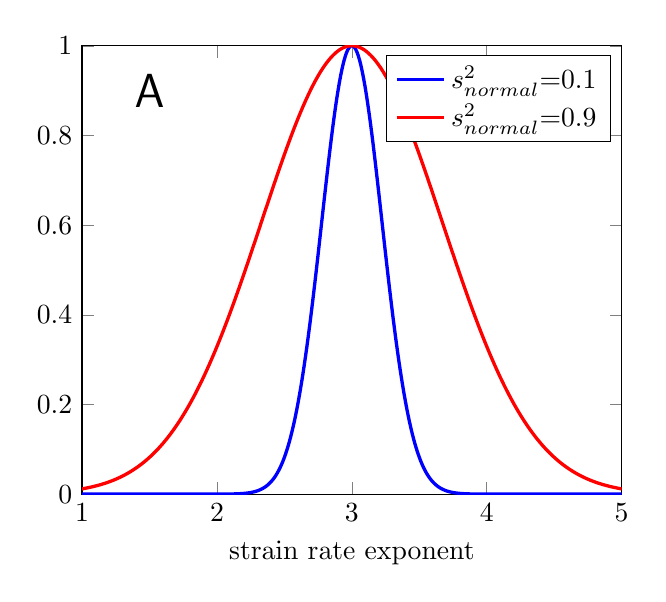
\begin{tikzpicture} 
\begin{axis}[ xlabel=strain rate exponent,xmin=1.0, xmax=5.0, ymin =0, ymax = 1.0 ] % invoke external gnuplot as % calculator: 
  \addplot [mark=none,very thick, blue, samples=1000]{exp(-(x-3.0)^2/0.1)}; 
  \addlegendentry{$s_{normal}^2$=0.1}
  \addplot [mark=none,very thick, red, samples=1000]{exp(-(x-3.0)^2/0.9)}; 
  \addlegendentry{$s_{normal}^2$=0.9}
\node[font=\fontsize{18}{18}\sffamily] at (axis cs:1.5,0.9){A};


\end{axis} 
\end{tikzpicture}
}
\hspace{-0.2cm}\subfigure{

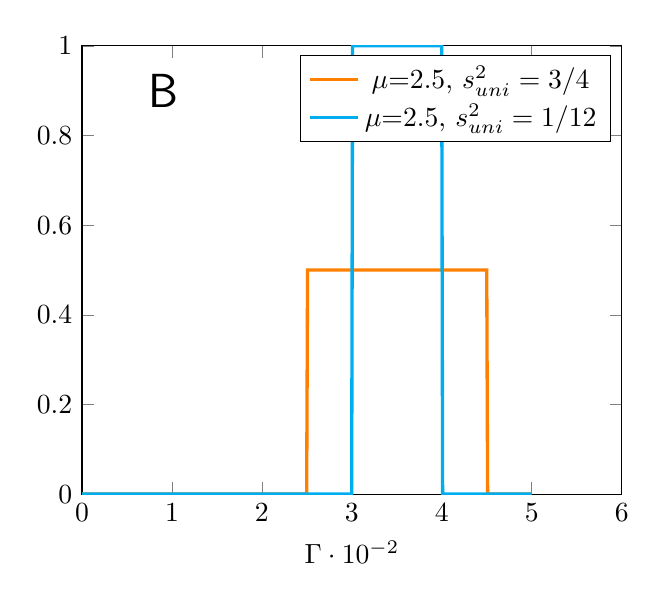
\begin{tikzpicture}[
    declare function={unipdf(\x,\xl,\xu)= (\x>\xl)*(\x<\xu)*1/(\xu-\xl);}
]
\begin{axis}[xlabel = $\Gamma \cdot 10^{-2}$,
    samples=1000,
%    const plot mark mid,
    xmin = 0, xmax = 6,
    ymin=0,ymax=1
]
\addplot [very thick, orange] {unipdf(x,2.5,4.5)};
 \addlegendentry{$\mu$=2.5, $s_{uni}^2 = 3/4$}
\addplot [very thick, cyan] {unipdf(x,3,4)};
 \addlegendentry{$\mu$=2.5,  $s_{uni}^2 = 1/12$}
\node[font=\fontsize{18}{18}\sffamily] at (axis cs:0.9,0.9){B};
\end{axis}
\end{tikzpicture}

}

\caption{(A) Normal distributions for the strain rate exponent prior (B) Uniform distributions for the strain rate exponent prior. In (A) we compare the possibility of using two different normal distributions to demonstrate our knowledge or lack thereof of what the values of the strain rate exponent should be. }
\label{fig:prior_ex} 
\end{figure}

\mgnote{Don't use $\sigma$ use $s$ as I suggested earlier.}\vrnote{done}Another possibility is to use a \textit{non-informative prior} \citep{Tarantola05} which gives gives equal likelihood (equal probability) to each value such that no preference is given to a single value. Using non-informative priors can be advantageous when it is not apparent what an acceptable value is, such as the strength of a weak factor An example of a non-informative prior is a uniform distribution for the strain rate exponent (Fig.\ref{fig:prior_ex}b). A uniform distribution has the following properties,
 \begin{align}
\mathcal{U}(a,b) =
\begin{cases}
 \frac{1}{b-a}   &b\geq x \geq a \\
               0 &\quad \text{otherwise} \\
\end{cases}
\end{align}
with a mean and variance of \mgnote{next two should be inline} \vrnote{done}
\begin{align}
\mu(a,b) =\frac{1}{2}(a+b) \quad s_{uni}^2(a,b) =\frac{1}{12}(b-a)^2 .\
\end{align}
The uniform distributions (Fig.~\ref{fig:prior_ex}b) have the same mean, but different variance. Compared to a normal distribution, the variance for the uniform distribution is determined by the range of likely values, each of which has the same probability.
	
 For a prior described by a normal distribution, a mean, $\mu$, and covariance, $\mathcal{C}$, are needed
\begin{equation}
\ppi_{prior} = \mathcal{N}(\mu,\mathcal{C})
\end{equation}
The negative log of the prior distribution results in a weighted misfit, or
\begin{equation}
\mathcal{J}_{prior} = \frac{1}{2}(\mm-\mm_{mean})^\intercal\mathcal{C}^{-1}(\mm-\mm_{mean})
\end{equation}
With the prior, the cost function would be
\begin{equation}
\begin{split}
  \mathcal{J}(\uu,\mm,p)&:= \frac{1}{2}\int_{\partial \Omega_1} (\mathcal{O}\uu-\uu_{\text{obs}})^\intercal\mathcal{C}^{-1}_{vel}(\mathcal{O}\uu-\uu_{\text{obs}})d\partial\Omega_1 \\
%  &+\frac{1}{2}(\eta_0 - \text{exp}({\int_{\Omega_i} \ln \eta}))^{2} \\
   &+(\eta_0 - \text{exp}({\int_{\Omega_i} \ln \eta}))^{2} +\frac{1}{2}(\mm-\mm_{mean})^\intercal\mathcal{C}^{-1}(\mm-\mm_{mean}).
\end{split}
\end{equation}
\mgnote{The second term on the rhs for the integral has a missing differential}\vrnote{done}While the solution to the adjoint equation does not change, the gradient term for each parameter becomes
\begin{equation}
\mathcal G:= \int_{\Omega} [2 \eta_{,i}(\IIinv, \Gamma, n, \sigma_y)\strain(\uu):\strain(\vv) d\Omega  + \mathcal{C}^{-1}(\mm-\mm_{mean})\mm_i d\mm].\
\end{equation}
These new gradients will be used to update the parameters as they measure the sensitivity of a parameter to an observation.


\section{Model Setup}
We have constructed a set of model constraints based on global observations with four components: A global temperature distribution, the geometry of faults, the kinematics of plate motion, and the geometry and bounds on the effective viscosity within selected regions.

The temperature model has been constructed globally in a spherical shell from which selected cross-sections are taken. The temperature of oceanic lithosphere follows a half-space cooling model using  updates to the digital grid of the age of the oceanic plates \citep{muller1997digital}.  
A thermal age was used within continental regions with the following three regions: Cratons (300 Ma), areas near subduction zones (75 Ma), and other areas (200 Ma), as detailed in \citep{Stadler27082010}.
The thermal structure of slabs were constructed as follows. 
Initially the top surface of the slabs was derived from the Slabs 1.0 surface, based on detailed seismic constraints, including seismicity and seismic reflection profiles \citep{Hayes2012}.
With normals pointing downward from this surface, an initial thermal structure of slabs based on the half space model using the age of the plate at the position of the trench was generated. This proceedure ensured continuity with the thermal structure of the oceanic lithosphere. Then, thermal conduction was solved for at each depth over a duration equal to the travel time to reach the depth with the local convergence velocity (using the relative velocity vector). Although solved only with conduction, this procedure resulted in thermal structures close to those obtained in fully dynamic models. The tops of thermal  slabs were sharp in the corner of the mantle wedge and then progressively became more diffusive with depth.
Within the lower mantle the thermal structure was based on scaled seismic tomographic models,
including a P-wave \citep{simmons2012llnl} and a S-wave model \citep{ritsema1999complex}.
The lithosphere and upper mantle models and the upper and lower mantle were blended together at 75 km and 550 km depths, respectively, as shown in cross sections (Fig.\ref{fig:xsection2sumatra}).
We have used the seismo-tectonic approach for the shallower mantle and tomographic approach for the deeper mantle, as the seismic tomography models for slabs tend to be noisy.


On the surface of the earth we generated a veloctiy field from MORVEL56 \citep{GGGE2060} in a no net rotation (NNR) reference frame. Each cross-sectional model generally defines a great circle arc, with local unit vector \textbf{d} in the direction of the circle, such that we extracted the velocity $v_{xs}=\textbf{d}\cdot\textbf{v}$.  The NNR reference frame was used as the side-walls on the two-dimensional cross sections preclude any large-scale differential motion between the bulk of the mantle and the plates.






\begin{figure}[hbtp]
\centering
\scalebox{1.6}{
\hspace{-1.8cm}\subfigure{
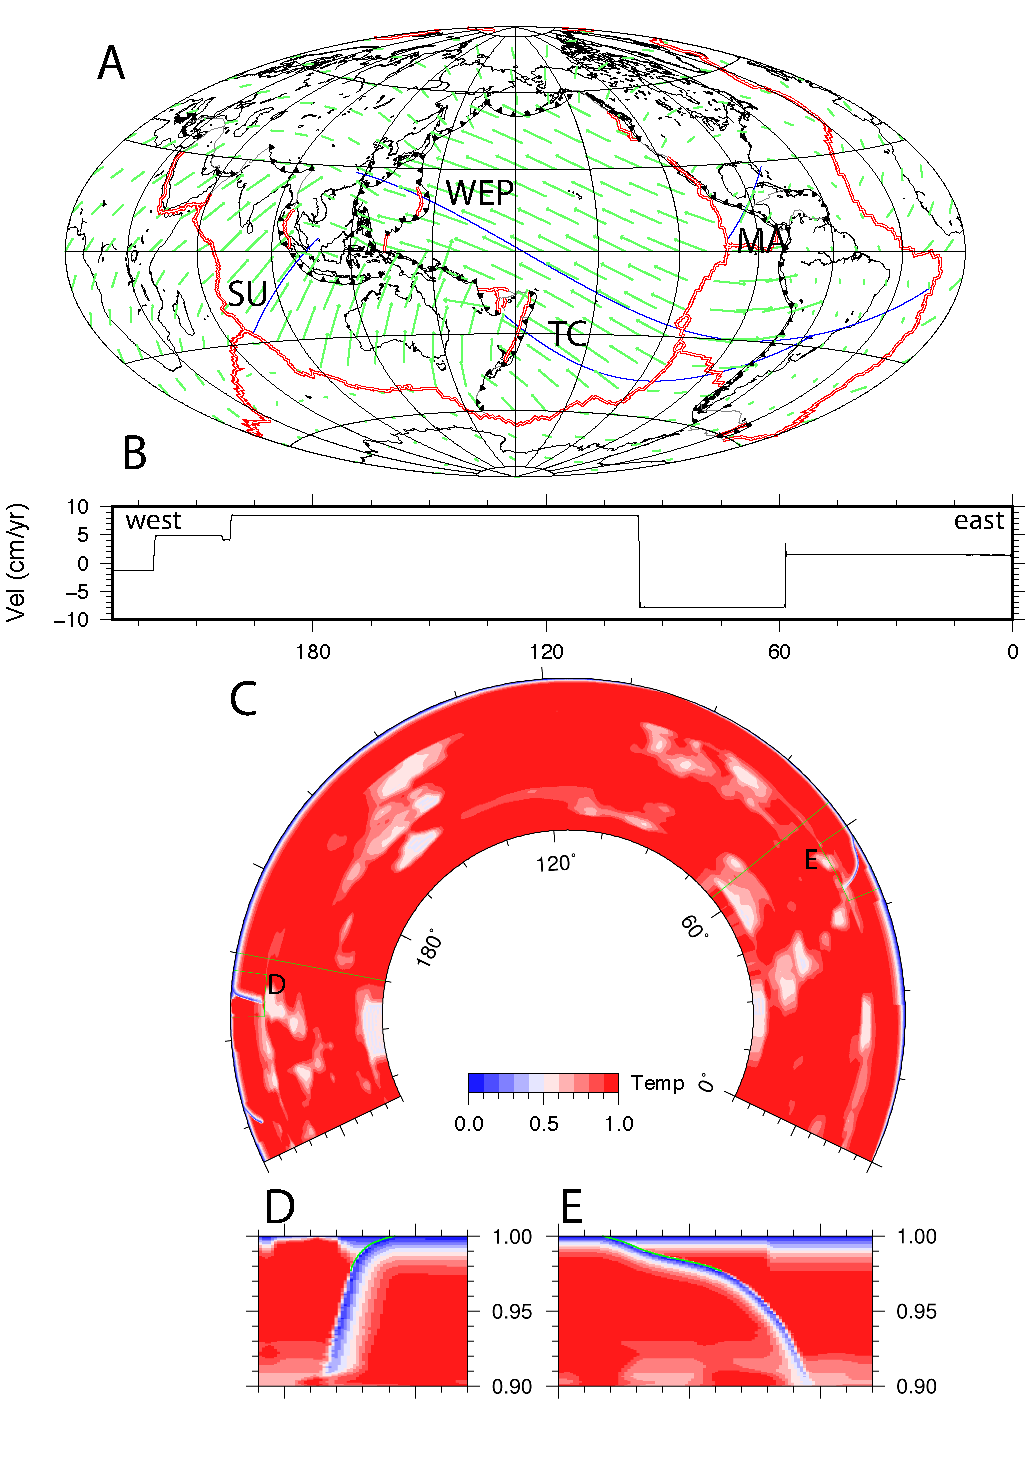
\includegraphics[height=150mm,width=100mm]{Summary_sections.pdf}%{mesh.pdf}
}

}

\label{fig:xsection2sumatra}
\end{figure}

\begin{figure}[hbtp]
\centering

\caption{\vrnote{should the caption have a sole page or should it just continue onto the next page?}\mgnote{I would put only the Figure on a seperate Figure and the Caption on an adjacent Page. This is commonly done for Caltech Thesis Style. This allows the Figure to be it's largest, which is essential as there is too much white-space the way it is.}A. Velocity vectors in the no net rotation reference frame. Cross sections indicated with black lines, including western to eastern Pacific (WEP), Sumatra (SU), Tonga to Chile (TC) and Middle America (MA) B. Velocity in the direction of cross-section WEP.(C)Temperature distribution for cross section WEP. Zoom in of the Marianas (in D) and the Chilean (in E) slabs for the WEP cross section. In D and E, the solid green lines show the position of the weak zones.}
\label{fig:caption}
\end{figure}



Selecting a set of representative cross-sections in which all of the driving forces may be represented two-dimensionally is difficult, as it is likely that no plate and subduction zone is truly two-dimensional. 
Nevertheless, we have chosen a set of cross-sections in which plate motion was generally orthogonally to the strike of the trench and which represent some of the end-member cases from the least to the most seismically coupled subduction zones (Fig.\ref{fig:xsection2sumatra}A). To investigate the coupling for various seismically coupled subduction zones, we consider the cross-sections in Fig. \ref{fig:xsection2sumatra}. 
Our primary cross-section has the largest dimension (about $240^{\circ}$, WEP, weatern to eastern Pacific) and contains three subduction zones that span the range from the seismically coupled (Chile) to the least coupled (Marianas). This cross section contains one subduction zone with back-arc extension. Additional cross-sections in Fig.\ref{fig:xsection2sumatra} are smaller than WEP, and thus do not contain the coupling variability of the larger cross-section; however those cross-sections represent subduction zones that exhibit both substantial coupling (Sumatra) and ittle coupling (Tonga).




The fault zone between converging plates at subduction zones, generally thought to be the places on which great earthquakes occur, were represented as weak zones with unknown viscosity. 
A weak zone factor, created by a stencil with a center line defined by the Slabs 1.0 surface \citep{Hayes2012}, was defined as
\begin{equation}
\Gamma_{stencil} = 1.0 - (1-\Gamma_i)\exp\{-(d_i-d_0)^2/(2\cdot w^2)\}
\end{equation}
and with a coefficient $\Gamma_i$ that was recovered in ~\eqref{eq:rheo}, $d_0$ is the center-line profile, $w$ is the length-scale of smoothing for the weak zone.
 For our models, we assume the values of mantle parameters summarized in Table ~\ref{table:parameters}.

\begin{table}[H]
  \caption{Assumed parameters left as constants in the }
  \centering  % used for centering table
  \begin{tabular}{c c c} % centered columns (2 columns)
    \hline \hline                        %inserts double horizontal lines
    Symbol & Parameter & Value  \\ [0.5ex] % inserts table
    %heading
    \hline                  % inserts single horizontal line
    $\rho$ & Density ($\rho$)  & 3300 kg/m$^3$ \\
    $g$ & Gravity ($g$) & 9.81 m/s$^2$ \\
    $\alpha$ & Coefficient of Thermal expansion ($\alpha$) & 2 $\times$ $10^{-5}$ \\ 
    $\Delta T$& Temperature Difference $\Delta T$ & 1400 K \\
    $D$& Depth of layer ($D$) & 1500 km \\
    $\kappa$& Thermal Diffusivity ($\kappa$) & $10^{-6}$  m$^2$/s \\
    $\eta_{\text{ref}}$& Reference Viscosity  ($\eta_{\text{ref}}$) & $10^{20}$ Pa $\cdot$ s \\
    Ra & Rayleigh Number (Ra) & 2.92 $\times$ $10^9$ \\
    $n$ & Strain rate exponent in lower mantle ($n$) & 1.0 \\
    \hline %inserts single line
  \end{tabular}
  \label{table:parameters} % is used to refer this table in the text
\end{table}

%\mgnote{\P~needs to be moved to the Discussion since in the end you do not factor in the uncertainty of your data. Move this \P, and then finish it with a discussion of how your method can be expanded in the future.} A caveat in these cross-section optimizations is that both the tomography model and plate motion data are not unique and therefore have implicit uncertainty embedded within. For example, there are multiple tomography models that can be used in the lower mantle, such as the shear-wave model S40RTs \citep{ritsema2011s40rts} or the P-wave model (LLNL-G3Dv3) \citep{simmons2012llnl}), while plate motion data is dependent on the reference frame used such as plate motions with respect to hotspots, with respect to a specific plate (Pacific for example), or the no-net-rotation(NNR) reference frame. 
%In addition to the uncertainty of the reference frame, there is uncertainty in the motion of one plate with respect to others which can possibly influence the parameter estimation of plate couplings. Therefore, while it is possible that the magnitudes of the rheological parameters may be different for different tomography and plate motion models, the overall relative (mechanical) coupling of subduction zones should not vary from those obtained from seismic coupling (\citep{scholz2012seismic}).


\mgnote{This is vague. The viscosity constraints need to be described in precise terms (e.g. magnetude of viscosity and geometry with reference citations}As presented earlier, the average effective viscosity data is an additional constraint that we will explore to determine the effect it has on the inference of the rheological parameters. Since the effective viscosity is a constraint on the mantle from observations, then this data should better constrain global parameters such as the strain rate exponent, activation energy, and upper mantle prefactors. We will place the average effective viscosity constraint of $\overline{\eta}_j = 10^{19} Pa\cdot s$ under the South American plate \mgnote{Why not $10^21$ Pa-s? We must discuss}, (as it is the only plate in our models with a substantial continental plate overriding a subduction zone), as well as underneath Japan with $\overline{\eta}_j = 10^{19} Pa\cdot s$ \citep{hu2016asthenosphere} \vrnote{i need to find the exact dimensions used}.\mgnote{The specific outlines of the constrain on the viscosity need to be shown}
 While we are able to solve this nonlinear Stokes flow, we need to resolve the thermal boundary layers and fault zones. Doing so requires either using small elements with uniform refinement, which would be computationally expensive. Therefore, we use adaptive mesh refinement (AMR) and refine in areas such as cold thermal boundary layers (oceanic plates) and fault zones (2 km resolution). 
We solve the nonlinear incompressible Stokes by linearizing the momentum equations, enabling the use of Newton's method \citep{rudi2015extreme}. 

\section{Results}

\mgnote{I haven't yet deleted the text I made earlier as I think that the Results section still needs a lot of work. In the UQ subsection there are parts where you are starting to give this physical understanding of the results, when it comes to the conditional distributions.}

\mgnote{Both of these sub-sections suffer from the same problem. You say we tried case x and we get y, but there is no discussion of the 'why'. This is geodynamics, we are in the business of providing answers on the 'why'. How can you arrive at these conclusions and discussions? You need to look at the equations, both of motion and  viscosity, perhaps plots of effective viscosity and then your conditional distrbutions. I will give a lot of commentary in the days ahead on improving in this regard.}

\subsection{Inversions}
Based on the numerical machinery that we have developed, look at what values of the rheological parameters that best fits the observed plate motions. Constraining those rheological parameters is important as it will provide an accurate balance of resisting forces within the plates. 
 Unlike our earlier studies \citep{ratnaswamy2015adjoint}, we do not know the true values of the rheological parameters. To make sure that we infer a set of parameters, we make sure that the misfit in plate potions is sufficicently minimized by reducing the norm of the gradient by three orders of magnitude. While, reducing the norm of the gradient is important, we need to test the sensitivity of the initial guess to determine if there are multiple minimas. Doing so, we test perturbing the initial strain rate exponent guess from 2.0 to 3.5  in Table \ref{table:initial_guess} and find that regardless of the initial guess of the strain rate exponent and show that we recover the same plate couplings, yield stress and strain rate exponent for the WEP cross-section. This result is important as it establishes that multiple inversions would not be needed to obtain as the inferred rheological parameters are the same independent of the initial guess. 
 
Establishing the stability of the inversions, we now systematically infer the rheological parameters for each cross-section, specifically the parameter ranges of the inferred strain rate exponent, yield stress and weakfactors (2)isolating what the parameter trade-offs are (3) how much the variance is minimized with additional viscosity data. Starting with the larger cross-section (WEP), we look at what the inferred parameters are solely due to the observations, without using priors oraverage viscosity data. We first begin by systematically varying what parameters to infer so as to ascertain what the tradeoffs are.  The main parameters that were explored in \citep{ratnaswamy2015adjoint} were the plate couplings, strain rate exponent, yield stress, activation energy and upper mantle prefactor in Cases 1-6. The range of inferred strain rate exponent lies within  3.047-3.09, which is approximately 1.67-2.67 $\%$ larger than the initiatl guess of 3.0. Furthermore, the infered strain rate exponent values suggest that there is more shear thinning in the upper mantle than what the initial state is, which further supports the claim that the upper mantle is governed by dislocation creep. 

The yield stress is an important parameter as it provides weakening in the hinge zone to relieve the large stresses as plates bend. The inferred yield stress we find is in the range of 129.5-146 MPa, which is 7.92-21.67 $\%$ increase from the initial yield stress. This increase in yield stress suggests that plates have less dynamic weakening in the initial state, however; there is still dynamic weakening occurring within the hinge zone as evidenced by the reduction in the effective viscosity. Furthermore, in Cases 1-6, the average effective viscosity in the hinge zone is approximately 7-9 $10^{21} Pa\cdot s$, regardless of which combination of the parameters are inferred, suggesting that there is a bounded effective viscosity in the hinge zone that best minimizes the misfit in observed plate motions and model results. An important trend in Cases 1-6 is that as the strain rate exponent increases, the yield stress increases, implying that there may be a correlation between both parameters. Looking at the conditional distributions in Fig., we find that there is a positive trade-off such that as the strain rate exponent increases (plate motions increase), the yield stress also increases (reducing plate motions) to compensate for a weaker upper mantle, a result that was also found in \citep{ratnaswamy2015adjoint}.

The plate couplings is an important part of our inferences as it tells us which plate boundaries have more shear resistance. In Cases 1-6, we find that there is a preferred ordering of the plate couplings, where South America is approximately two orders of magnitude larger than Ryukyu and Izu-Bonin. Furthermore, the values are fairly constant and generally fluctuate, which also suggests that these values generally are bounded, even without prior knowledge. The relationship between the plate couplings and yield stress are found in the conditional distribution in Fig. where we find for each subduction zone in WEP, there is a negative correlation between the plate couplings and the yield stress. This correlation can be explained due to an increase in coupling will reduce plate motions, which will promote more dynamic weakening in the form of reducing the yield stress, so as to increase plate motions. Analyzing the relationship between the plate couplings and strain rate exponent, we similarly find that there is a positive correlation between the strain rate exponent as expected due to an increase in plate coupling (decrease in plate motions) which requires an increase in the strain rate exponent to increase plate motions.  An important observation from the conditional distributions is that there is a partitioning of the plate couplings for Izu-Bonin, Ryukyu and South America, where Izu-Bonin and Ryukyu are grouped together on the decoupled spectrum, while South America is more on the coupled side.  

Two new parameters that we inferred in these studies are the upper mantle prefactor and the activation energy. Both parameters control aspects of the viscosity contrast between the plates and the upper mantle. For example, increasing the upper mantle prefactor would increase the viscosity of the upper mantle, which would in turn reduce the viscosity jump between the upper and lower mantle. The activation energy would increase or decrease the viscosity contrast between the slabs and the mantle, and therefore plays a crucial role in ascertaining how strong slabs are.  Therefore, we examine the role of both these parameters on the plate couplings, yield stress and strain rate exponent. In an extreme case, we infer all the parameters in Case 6 and find that the pattern of South America having a larger plate coupling than Ryukyu and Izu-Bonin remains the same, suggesting that the plate couplings are independent of the global rheological parameters. We also find that when there is an increase in the activation energy, there also is an increase in the upper mantle prefactor which suggests that the viscosity contrast between the upper mantle and slabs is compensated by increasing the upper mantle prefactor. 

While we inferred the rheology without knowledge and obtained important trade-offs between the rheological parameters, we need to reduce the uncertainty (variance) of the inferred parameters, which requires the use of priors and additional pieces of data. Introducing prior knowledge into our inversions, we us Gaussian priors for each of the inferred parameters, as shown in Table - making sure that we do not restrict the likelihood to a particular parameter space, that is not allowing out knowledge to influence the likelihood distribution strongly.  We repeat similar inversions in Cases 7-10, that were done in Cases 1-6 so as to ascertain if the correlations between the paramters remain (2)how does the \textbf{MAP} point change. Overall, we find that the correlations remain the same, that is there is a positive correlation between the strain rate exponent and yield stress remains. Furthermore, we find the ordering of plate couplings is the same, where South America is more coupled than Izu-Bonin and Ryukyu. With regard to the convergence of the parameters, we find that there is similar convergence to without using priors in Fig. (approximately 7 iterations).

Using priors is standard for parameter inferences, an important result would be how the inferred global parameters such as the strain rate exponent, and activation would change when using average effective viscosity data is used, that is how much the variance of those parameters are minimized, and is the rate of convergence different from using priors. In Cases  , we find that that the rate of convergence is the same compared to Cases where priors were used (approximately 7 iterations), which is similar to Cases 1-10, where priors were not used. The plate couplings are similar to what was found previously, while the ordering is the same, suggesting that there is a preferential relative coupling for subduction zones. When examining the the correlations between the inferred parameters, we find that the strain rate exponent still has a positive correlation with the the yield stress, while the plate couplings are still exhibiting a negative correlation, signifying that with additional data, the underlying correlations remain due to the physics of the nonlinear Stokes flow system. 

In a similar vain, we now enforce both priors and the average effective viscosity data to further minimize the variance of the inferred rheological parameters. Doing so will enable us to test if the priors and additional effective viscosity data would preserve the correlations between the rheological parameters. Doing so, we note a similar rate of convergence, where we reduce the norm of the gradient sufficiently compared to Cases 1-20. The inferred values are similar to what was found in previous cases; however, we find that the variances, are further minimized when looking at the conditional distributions, while the correlations remain the same. This result is indicative that we have not set strong priors, but rather allowed for the data to inform the parameters. 

While WEP represents a large cross-section with subduction zones with various seismic coupling, what would happen if we were to focus on a sole subduction zone, if the parameters would be the same. Therefore, we repeat similar experiments as was done with WEP to see how the inferred parameters differ and if the same trade-offs exist. Similar to WEP, we repeat the same experiments where we we let the data decide what the parameters should be. Doing so, we find that when using plate motions, we find that similar to what was found in WEP, the inferred strain rate exponent is larger than the initial guess, more specifically, we find in Case 15 that the plate coupling is larger than what was found in Ryukyu and Izu-Bonin. Furthermore, the yield stress that was inferred is 143.1 MPa, which is in line with what was inferred for WEP, while holding the activation energy and upper mantle prefactor fixed. When the parameters are allowed to be unconstrained and we now infer all the parameters such as strain rate exponent, yield stress, plate coupling, upper mantle prefactor and activation energy. Inferring all the parameters in Case 16, we find that the strain rate exponent is 3.11, which is larger than what was inferred for WEP, while the yield stress is 141 MPa, which was similar to what was inferred in Case 15 for Sumatra. The plate coupling that was inferred is less than what was inferred in Case 15, however; the decrease in plate coupling could be due to an increase in plate coupling, which was found in the conditional distributions. The inferred activation energy for Sumatra in Case 16, is larger than the initial guess, a result that was similarly found for the cases in WEP, which suggests that when the parameters are unconstrained, the system prefers a stronger temperature dependent rheology. The increase in activation energy also brings about an increase in the upper mantle prefactor, which is a parameter that increases the effective viscosity as that parameter increases. 

To address the activation energy value that was inferred in Case 16, we now fix the upper mantle prefactor to see what the impact would be on the activation energy. Doing so, we find that the plate coupling is lower that what was found in Cases 15-16; however, the value is still larger than what was inferred from WEP. The strain rate exponent and yield stress are lower than what was found for Sumatra in Cases 15-16, while the activation energy is lower than what was inferred in Case 16, where all parameters were inferred. The reduction in the inferred activation energy with regard to Case 16 can be attributed to keeping the upper mantle prefactor fixed (less than the inferred value in Case 16), which would require less temperature dependence on the effective viscosity. We continue to hold certain parameters fixed to isolate the trade-offs among other parmaeters. In Case 18, we fix the strain rate exponent, and infer the rest of the parameters. We find that the yield stress is lower than what was found in Cases 15-17, which can be due in part to the fixed value of the strain rate exponent (reduced from the inferred values). Furthermore, the plate coupling is also reduced from Case 17, which can be caused due to a lower yield stress, which causes more weakening. While, the yield stress and plate coupling have decreased, we find that the activation energy and upper mantle prefactor have increased similar to what was found in Case 16, which suggests that there may exist a strong connection between these global parameters. Similar to Case 18, we now fix the yield stress and infer the rest of the parameters, and find that there is an increase in the plate coupling with the increase in strain rate coupling. Furthermore, there is an increase in both the activation energy and upper mantle prefactor which furthermore suggests that both of these parameters are strongly correlated.  

While we used data to infer the parameters for Sumatra, we need to look at how using priors can help reduce uncertainty as it did for WEP to determine if the correlations hold for different parameters. We find in Case 20, we find that when conditioning on the upper mantle prefactor and the activation energy, the strain rate exponent is larger than 3, further suggesting that the the inferences suggest that upper mantle is dominated by shear thinning. When allowing all the parameters to be inferred, we find that the strain rate exponent is larger than Case 20, while the activation energy and upper mantle prefactor increased. The increase in he upper mantle prefactor coincides with an increase in the activation energy, which can be explained due to the increase in viscosity variations from an increase in the activation energy, which in turn requires an increase in the upper mantle prefactor to compensate for that increase. Furthermore, the increase in upper mantle prefactor can precipitate an increase in the strain rate exponent so as to compensate for the increase in viscosity. When conditioning on either the strain rate exponent (Case 23) or yield stress (Case 24), we find that the plate coupling decreases from Cases 20 and 21 when those two global parameters were not fixed.

In a similar vein, we investigate the Tonga subduction zone using data and priors. We find that the inferred plate coupling for Tonga is lower on average for cases with (28-31) and without priors (24-27). This result is indicative of Tonga preferring a more decoupled plate boundary than South America and Sumatra, regardless of prior knowledge. We find that we do not impose priors, we infer a strain rate exponent larger than the initial guess for Cases 24-27. However, these values  do fluctuate depending on the number of parameters to be inferred, that is when the number of parameters increase, the strain rate exponent tends to be larger. Overall, we find that the average effective viscosity in the weakzone is consistently the same, with an average value of $8.52 \pm 0.17 Pa \cdot s$, suggesting that regardless of which combination of parameters are inferred the average effective viscosity value within the hinge zone is conserved. 

We end our analysis at the Central America subduction zone, where we compare how the plate coupling and global rheological parameters are similar or different to the previous cross-sections. One of the main results we find from Central America whether we impose or do not impose priors, the plate coupling is smaller than South America in WEP and Sumatra, while larger than Tonga in Cases 32-39, indicative of a preferential ordering of plate couplings among the cross-sections. Furthermore, in the absence of priors and all the parameters are inferred in Case 33, we find that there is an increase in strain rate exponent (about 1.89$\%$) compared to what was inferred when the activation energy and upper mantle prefactor were fixed in Case 32. Furthermore, we see a similar pattern to previous cross-sections where if either the strain rate exponent or yield stress is held fixed, the inferred strain rate exponent or yield stress is smaller than if both were inferred. For comparison, when we impose priors, we have an overall reduction in the strain rate exponent in Case 38, where all the parameters are free; however, the reduction in strain rate exponent still is larger than if some of the parmaeters are fixed in Case 32-33.

While, we see a pattern of which involves a partitioning of the plate couplings, a natural question to ask would be what if any overall changes would there be to the average viscosity in the uppermantle due to the nonlinear nature of the rheology. We find that overall, the average effective viscosity between all cases are $\mathcal{\O}(21)$; however, the values do fluctuate on a case by case basis per cross-section. For WEP, we find that the average effective viscosity in the upper mantle to be in the range of $2.29-4.57 \cdot 10^{21}Pa\cdot s$, suggesting that depending on the inferred value of the global rheological parameters (upper mantle prefactor, strain rate exponent), the average effective viscosity can increase if the strain rate exponent is small enough such that there is a dampening of shear thinning when there is an increase in the upper mantle prefactor. Looking at the smaller cross-sections we find that for Sumatra, there is a similar range of average effective viscosity in the upper mantle $[1.94,3.97]\cdot 10^{21}Pa\cdot s$ with the lower bound having a , which has a smaller upper bound than that of WEP. Similarly, we observe similar average effective viscosity ranges for Tonga ($[1.93,3.93]\cdot 10^{21}Pa\cdot s$) and Central America ($[1.89,3.15]\cdot 10^{21}Pa\cdot s$), suggesting that even though 


\begin{sidewaystable}

\centering

	\begin{table}[H]
		\caption{Case study summary\mgnote{ADD Footnote "Bold values are held fixed during the optimization"; "WEP: Western to eastern Pacific". Priors and visc data need to be seperate columns. It would be helpful (no essential) to have seperate collumns which give the effective viscsoity of both the upper mantle and the hing zone. Probably need a small Font to get everything in one Table }} % title of Table
		\centering  % used for centering table
        \scalebox{0.4}{
		\begin{tabular}{c c c c c c c c c c c c c c c c } % centered columns (2 columns)
		\hline \hline                        %inserts double horizontal lines
		Case & Subduction Zone & \textit{n} &$\sigma_y$&$\Gamma$ (SAM/RYU/IZU) $\cdot 10^{-5}$ &UM Prefactor &$E_a (kJ/mol)$&Visc. data   & Prior & Average $\eta_{UM} (10^{21})$  & $\eta_{hinge} (10^{21})$ & $\text{Drag Force} (10^{12}N/m)$ &  $\text{Slab Pull Force} (10^{12}N)$ &  $\text{Slab Shear Force} (10^{12}N/m)$ &  $\text{Bending Force} (10^{12}N)$ &  $\text{Fault Shear Force} (10^{12}N/m)$ \\ [0.5ex] % inserts table
		%heading
		\hline                  % inserts single horizontal line
         1 &WEP& 3.079 & 137 & $62.4/0.711/0.742$ & \textbf{2000} & \textbf{203.5} & no & no & 3.96 & $7.59/8.71/8.07$\\
         2 &WEP& 3.072 & 139 & $64.7/0.702/0.781$ & \textbf{2000} & 198.5 & no & no & 2.98 &$7.44/8.84/8.01$\\
        3 &WEP& 3.09 & 143 & $69.7/0.773/0.798$ & 2098.9 & \textbf{203.5} & no & no & 4.47 &$7.40/8.31/7.97$\\
        4 &WEP& \textbf{3.0} & 129.5 & $63.3 /0.703/0.725$ & \textbf{2000} & \textbf{203.5} & no & no & 4.57 &$7.49/8.81/8.17$\\
         5 &WEP& 3.047 & \textbf{120} & $73.9/0.681/0.733$ & \textbf{2000} & \textbf{203.5} & no & no & 3.11 &$7.38/8.89/8.13$\\
         6 &WEP& 3.066 & 141 & $69.8/0.656/0.745$ & 3019.1 & 232.7 & no & no & 2.29 &$7.42/8.80/8.11$\\
     7 &WEP& 3.051 & 146 & $72.3/0.744/0.791$ & \textbf{2000} & \textbf{203.5} & no  &yes &6.65 & $7.27/8.41/8.05$\\
        8 &WEP& 3.039 & 137 & $76.1/0.692/0.71$ & \textbf{2000} & 217.7 & no   &yes &4.51 &$7.25/8.92/8.23$\\
        9 &WEP& \textbf{3.0} & 139 & $60.1/0.655/0.733$ & \textbf{2000} & \textbf{203.5} & no  &yes &4.43 &$7.48/8.89/8.14$\\
         10 &WEP& 3.055 & \textbf{120} & $65.1/0.711/0.761$ & \textbf{2000} & \textbf{203.5} & no  &yes &4.62 &$7.43/8.73/8.12$\\
         12 &WEP& 3.052 & 143 & $70.7/0.735/0.81$ & 3471.4 & 230.4 & yes  &no & 4.73 &$7.40/8.74/8.11$ \\
         13 &WEP& 3.042 & 137 & $72.1/0.709/0.767$ & \textbf{2000} & \textbf{203.5} & yes  &yes & 3.79 &$7.37/8.79/8.14$ \\
         14 &WEP& 3.047 & 135 & $69.8/0.726/0.799$ & 4293.8 & 247.9 & yes  &yes &3.01 &$7.49/8.82/8.08$ \\
         15 &Sumatra& 3.087 & 143.1 & $63.9$ &  \textbf{2000}& \textbf{203.5}& no &no &3.61 & $7.79$  & $1.17$ & $64.7$ & $1.71$ & $48.9$ & $1.4$  \\
         16 &Sumatra& 3.11 & 141 & 44.1 & 3881.4 & 239.2   &no &no &2.81 & $7.87$ & $1.25$ & $64.7$ & $1.73$ & $49.3$ & $1.4$\\
         17 &Sumatra& 3.077 & 137 & 38.2 & \textbf{2000} & 200.1   &no &no &2.04 &$7.89$ & $1.21$ & $64.7$ & $1.81$ & $46.6$ & $1.5$\\ 
         18 &Sumatra& \textbf{3.0} & 129 & 30.7 & 2399.1 & 229.4   &no &no &3.97 &$7.78$&  $1.37$ & $64.7$ & $1.64$ & $44.2$ & $1.4$ \\
         19 &Sumatra& 3.077 & \textbf{120} & 41.7 & 2604.3 & 227.6   &no &no &1.89 &$7.88$ & $1.39$ & $64.7$ & $1.49$ & $47.1$ & $1.5$  \\
         20 &Sumatra& 3.048 & 143.1 & $63.9$ &  \textbf{2000}& \textbf{203.5}& no &yes &3.61 &$7.51$ & $1.42$ & $64.7$ & $1.67$ & $48.1$ & $1.4$   \\
         21 &Sumatra& 3.1 & 138 & 40.3 & 3394.1 & 231.4   &no &yes &1.94 &$7.85$ & $1.17$ & $64.7$ & $1.54$ & $48.7$ & $1.5$  \\
         22 &Sumatra& \textbf{3.0} & 128.1 & 38.2 & 2000 & 203.5   &no &yes &3.07 &$7.88$ & $1.31$ & $64.7$ & $1.71$ & $46.4$ & $1.5$ \\
         23  &Sumatra& 3.063 & \textbf{120} & 34.8 & 2302.6& 227.4   &no &yes &3.55 & $7.90$ & $1.42$ & $64.7$ & $1.63$ & $48.7$ & $1.6$\\
         24&Tonga  & 3.0621 & 139.1 & 0.63 & \textbf{2000} & \textbf{203.5} &no &no &2.89 & $8.59$ \\             
         25 &Tonga  & 3.051 & 135.2 & 0.7& 3196.1 & 225.8 &no &no &3.07& $8.53$ \\             
          26 &Tonga  & 3.087 &  \textbf{120} & 0.83 & 2000 &219.1  &no &no &3.55 & $8.41$\\              
          27 &Tonga  & \textbf{3.0}  & 127.7 & 0.67 & 3441.7 &232.7  &no &no &2.89 & $8.49$ \\             
          28 &Tonga  & 3.076 & 139.1 & 0.74& \textbf{2000} & \textbf{203.5} &no &yes &3.97 &$8.45$  \\          
           29 &Tonga  & \textbf{3.0} & 135.2 & 0.61& 3014.9 & 217.4 &no &yes &3.14 &$8.49$ \\             
          30&Tonga  & 3.097 &  \textbf{120} & 0.73 &3639.7 &228.3  &no &yes &3.29& $8.40$  \\             
           31 &Tonga  & 3.083  & 142 & $0.79 $ & 3492.3  &225.8  &no &yes &1.93  & $8.39$ \\             
            32 &Central America  & 3.0621 & 139.1 & 1.1& \textbf{2000} & \textbf{203.5} &no  &no &3.1 & $8.95$ & $1.77$ & $73.8$ & $2.14$ & $31.7$ & $1.26$\\               
            33 &Central America  & 3.12 & \textbf{120} & 0.83& \textbf{2000} & 178.1 &no &no &1.89 & $8.9$ & $1.77$ & $73.8$ & $2.08$ & $32.4$ & $1.21$\\       
            34 &Central America  & \textbf{3.0} & 132.1 & 0.92& \textbf{2000}& 207.2 &no &no &4.29 & $8.86$ & $1.79$ & $73.8$ & $2.16$ & $32.7$ & $1.15$  \\      
            35 &Central America  & 3.0 & 132.1 & 0.92& 2000& 207.2 &no &no &4.29 & $8.86$&  $1.71$ & $73.8$ & $2.24$ & $34.1$ & $1.23$  \\     
            36 &Central America  & 3.084 & 140 & 2.73& 4091.4 & 241.8 &no  &no &3.11 & $8.73$ & $1.73$ & $73.8$ & $2.17$ & $33.5$ & $1.27$\\                           37 &Central America  & 3.089 & 141 & 1.94& \textbf{2000} & \textbf{203.5} &no  &yes & 3.15 & $8.79$ & $1.795$ & $72.1$ & $2.26$ & $31.1$ & $1.19$\\              
           38 &Central America  & 3.092 & 143 & 1.06& 3471.3 & 233.7 &no  &yes &2.98 &$8.87$ & $1.73$ & $73.8$ & $2.19$ & $34.8$ & $1.21$\\       
           39 &Central America  & 3.092 & 143 & 1.06& 3471.3 & 233.7 &no  &yes &2.98 &$8.87$ & $1.71$ & $73.8$ & $2.21$ & $32.2$ & $1.29$\\             
                \hline %inserts single line
		\end{tabular}
        }
		\label{table:inversions} % is used to refer this table in the text
		\end{table}
\end{sidewaystable}


\begin{equation}
F_{drag} = \int \textbf{T}\ssigma \cdot \textbf{n} dl
\end{equation}

\begin{equation}
F_{slabshear} = \int \textbf{T}\ssigma \cdot \textbf{n} dl_{slab}
\end{equation}

\begin{equation}
F_{slabpull} = \int g\delta \rho \alpha dV
\end{equation} 
 
\begin{equation}
F_{bend} = \int \ssigma_{II} dA
\end{equation} 

\begin{equation}
F_{fault} = \frac{1}{\text{trench depth}}\int \textbf{T}\ssigma\cdot\textbf{n} dA
\end{equation} 
 
\begin{table}[H]
		\caption{Force Distribution} % title of Table
		\centering  % used for centering table
         \scalebox{0.5}{
		\begin{tabular}{ c c c c c c c c } % centered columns (2 columns)
		\hline \hline                        %inserts double horizontal lines
		 Subduction Zone &  $\text{Drag Force} (10^{12}N/m)$ &  $\text{Slab Pull Force} (10^{12}N/m)$ &  $\text{Slab Shear Force} (10^{12}N/m)$ &  $\text{Bending Force} (10^{12}N/m)$ &  $\text{Fault Shear Force} (10^{12}N/m)$   \\ [0.5ex] % inserts table
		%heading
		\hline                  % inserts single horizontal line
          Sumatra & $1.17$ & $7.37$ & $1.71$ & $3.14$ & $1.4$  \\
         Sumatra&  $1.25$ & $7.37$ & $1.73$ & $3.01$ & $1.4$\\
         Sumatra&  $1.21$ & $7.37$ & $1.81$ & $2.98$ & $1.5$\\ 
        Sumatra& $1.37$ & $7.37$ & $1.64$ & $2.99$ & $1.4$ \\
         Sumatra& $1.39$ & $7.37$ & $1.49$ & $3.12$ & $1.5$  \\
         Sumatra&  $1.42$ & $7.37$ & $1.67$ & $3.02$ & $1.4$   \\
        Sumatra & $1.17$ & $7.37$ & $1.54$ & $3.01$ & $1.5$  \\
        Sumatra&  $1.31$ & $7.37$ & $1.71$ & $3.15$ & $1.5$ \\
       Sumatra&  $1.42$ & $7.37$ & $1.63$ & $3.02$ & $1.6$\\   
        Central America  & $1.77$ & $8.47$ & $2.14$ & $2.55$ & $1.26$\\               
            Central America  &  $1.77$ & $8.47$ & $2.08$ & $2.57$ & $1.21$\\       
            Central America   & $1.79$ & $8.47$ & $2.16$ & $2.55$ & $1.15$  \\      
            Central America   & $1.79$ & $8.47$ & $2.16$ & $2.49$ & $1.15$  \\      
            Central America  &  $1.71$ & $8.47$ & $2.24$ & $2.51$ & $1.23$  \\     
            Central America  & $1.73$ & $8.47$ & $2.17$ & $2.57$ & $1.27$\\                          
            Central America   & $1.795$ & $8.47$ & $2.26$ & $2.45$ & $1.19$\\              
          Central America  & $1.73$ & $8.47$ & $2.19$ & $2.44$ & $1.21$\\       
          Central America   & $1.71$ & $8.47$ & $2.21$ & $2.48$ & $1.29$\\            
                \hline %inserts single line
		\end{tabular}
        }
		\label{table:initial_guess} % is used to refer this table in the text
		\end{table}




\begin{table}[H]
		\caption{Sensitivity of initial guesses for Case 1} % title of Table
		\centering  % used for centering table
		\begin{tabular}{ c c c c } % centered columns (2 columns)
		\hline \hline                        %inserts double horizontal lines
		 $n_{guess}$ &$n_{infer}$ &$\sigma_y$&$\Gamma $(SAM/RYU/IZU) $\cdot 10^{-5}$   \\ [0.5ex] % inserts table
		%heading
		\hline                  % inserts single horizontal line
        	 2.0 &3.042 & 146 & $99.2/0.81/0.772$   \\
	         2.95 &3.042 & 148 & $100/0.82/0.77$\mgnote{Is "100" a bound?}    \\
	         2.98 &3.046 & 146 & $67.3/0.773/0.798$  \\
	        3.5 &3.042 & 146.3 & $99.4/0.811/0.771$  \\             
                \hline %inserts single line
		\end{tabular}
		\label{table:initial_guess} % is used to refer this table in the text
		\end{table}
\mgnote{Specifically, is the effective viscosity before you add this additional constraint larger or smaller than the effective viscosity constraint? Look at this for both the whole upper mantle as well as in the specific area that the effective viscosity constraint is added.}



\begin{table}[H]
		\caption{Linear Viscosity role} % title of Table
		\centering  % used for centering table
		\begin{tabular}{c c c  c} % centered columns (2 columns)
		\hline \hline                        %inserts double horizontal lines
		$\eta_{diff}$&$\sum F_{shear}$boundary forces $10^{13}$& Slab Force$10^{13}$ & Difference $10^{13}$   \\ [0.5ex] % inserts table
		%heading
		\hline                  % inserts single horizontal line
        	0 & $14.05 $&$15.62$ & $1.57$   \\
        	1 & $14.53$&$15.62$ & $1.09$   \\
	        2 & $14.89$&$15.62$ & $0.73$   \\
	        3 & $15.55$&$15.62$ & $0.07$   \\
	        4 & $15.59$&$15.62$ & $0.03$   \\
 
                \hline %inserts single line
		\end{tabular}
		\label{table:parameters} % is used to refer this table in the text
		\end{table}



  % The first case study is shown below in Fig.\ref{fig:inverse1}
\begin{figure}[H]
\centering

\hspace{-0.2cm}\subfigure{
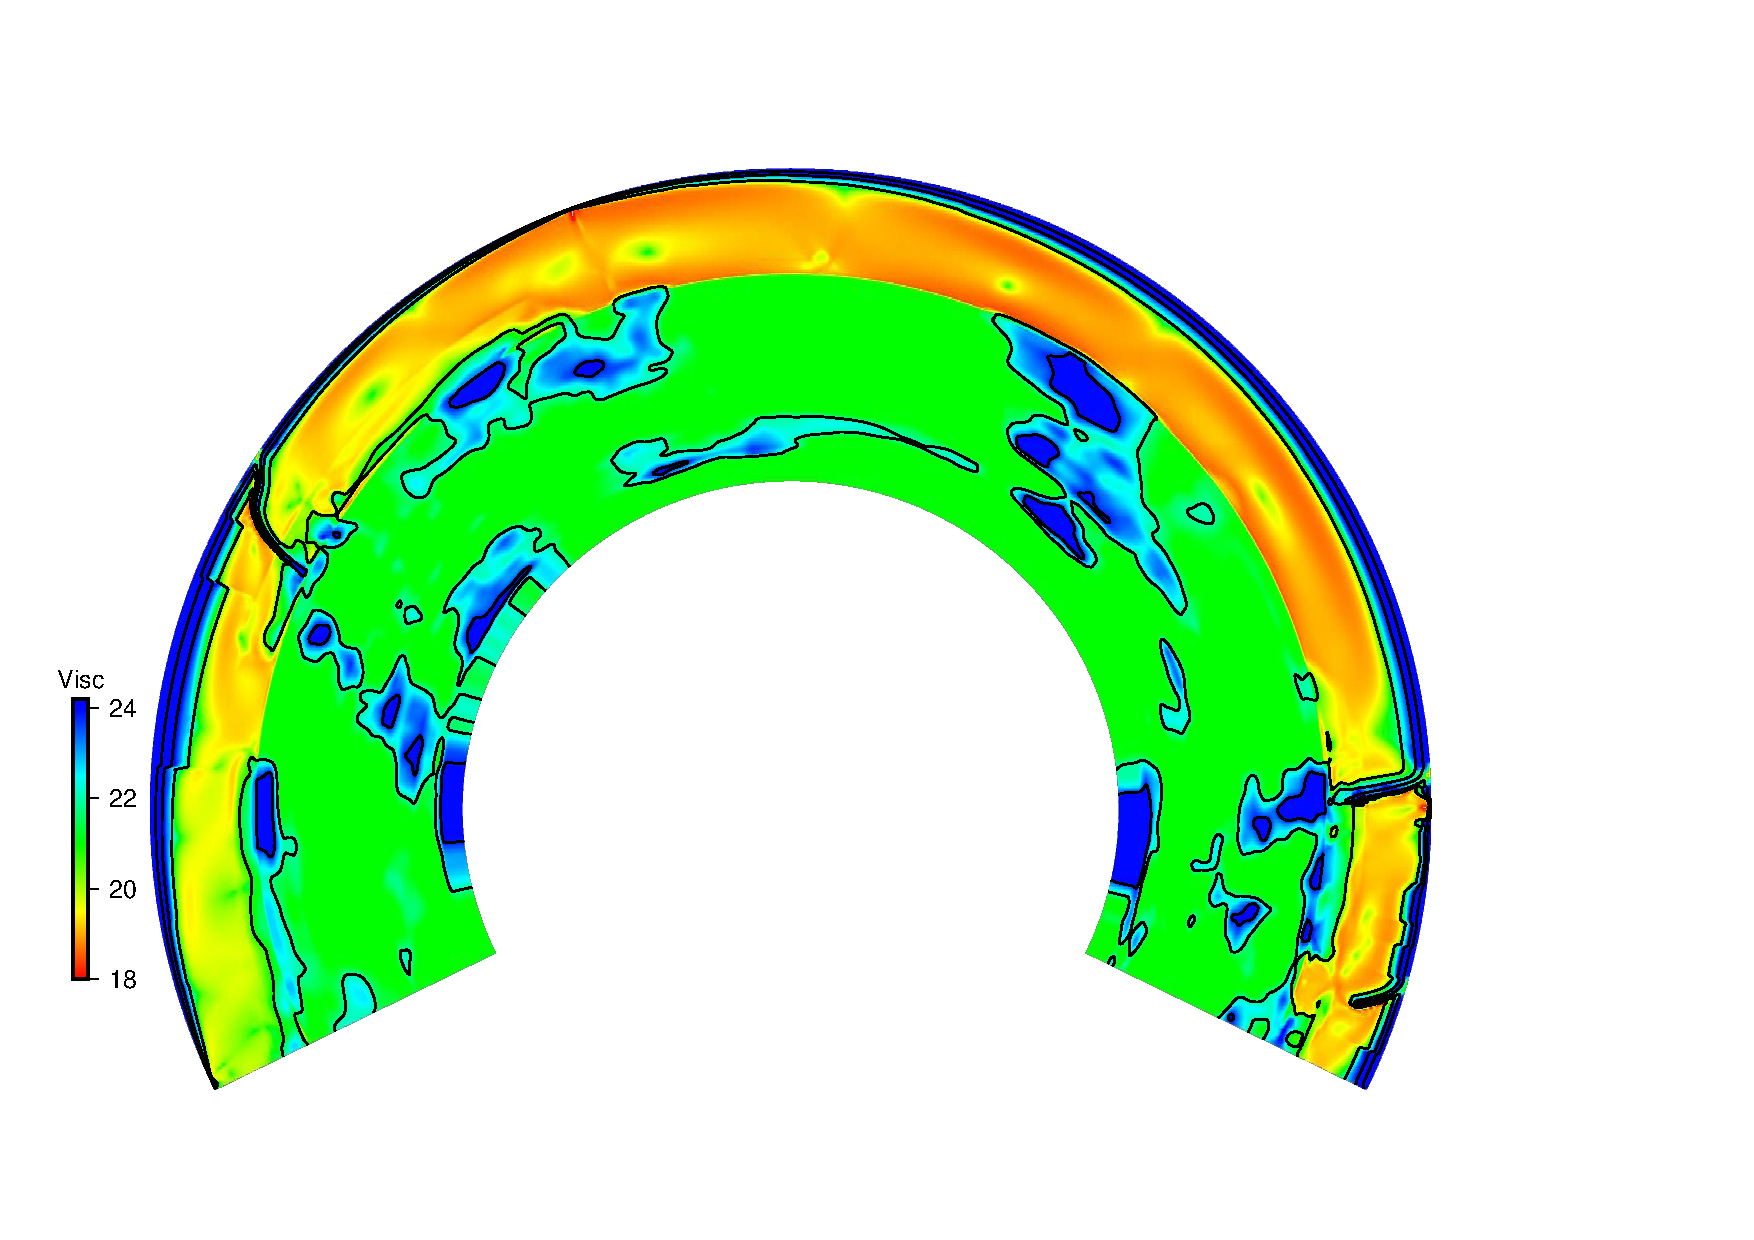
\includegraphics[height=65mm,width=128mm]{vish_contour.pdf}%{mesh.pdf}
}
\hspace{-0.4cm}\subfigure{
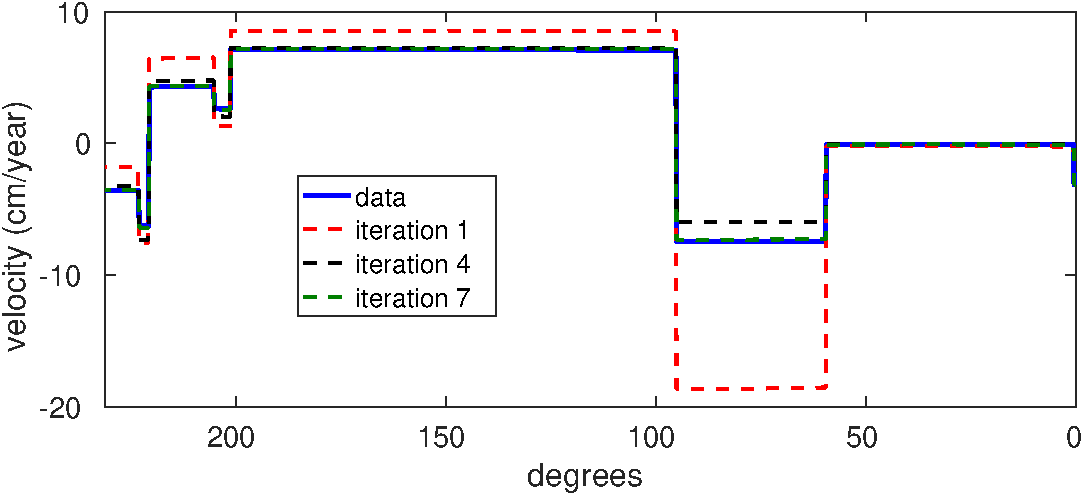
\includegraphics[height=35mm,width=58mm]{data_morvel.pdf}%{mesh.pdf}
}
\hspace{-0.2cm}\subfigure{
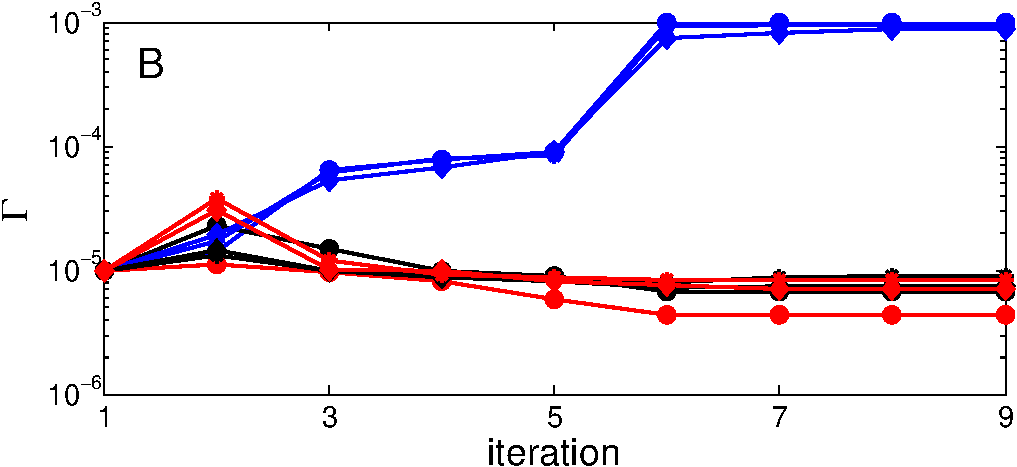
\includegraphics[height=35mm,width=58mm]{fig3b.pdf}%{mesh.pdf}
}
\hspace{-0.4cm}\subfigure{
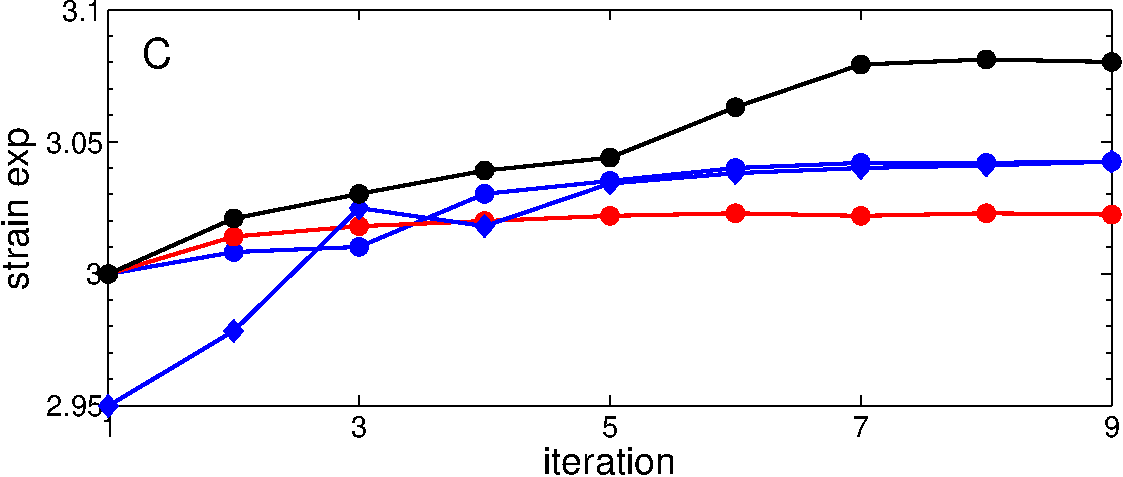
\includegraphics[height=35mm,width=58mm]{fig3c.pdf}%{mesh.pdf}
}
\hspace{-0.2cm}\subfigure{
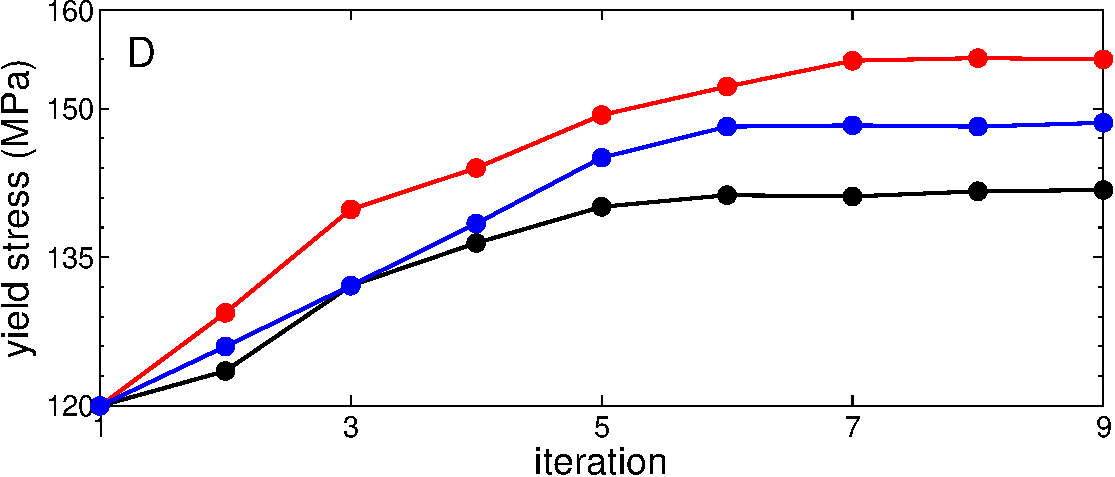
\includegraphics[height=35mm,width=58mm]{fig3d.pdf}%{mesh.pdf}
}
%\hspace{-0.2cm}\subfigure[]{
%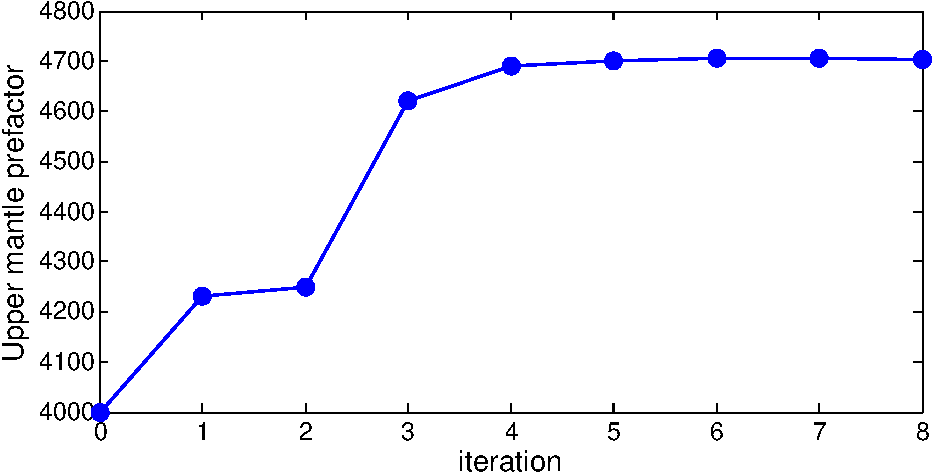
\includegraphics[height=35mm,width=58mm]{um_chap4.pdf}%{mesh.pdf}
%}

\caption{\mgnote{The labels in the Figure don't correspond with those in the Caption.}
(A) Effective viscosity for Case 1. \mgnote{Distance is flipped compared to Fig. 2C. Also the aspect ratio is messed upi -- it is stretched horizontally.}
(B) Surface velocity comparison between data and different iterations (Case 1). \mgnote{We need a zoom in on the velocity near the back-arc basin. This could be made a as an "insert". Please come by and see me for what I mean.}
(C) Plate boundary weakfactor iteration: South America (blue lines), Izu-Bonin (red lines), Ryukyu (black lines), with \textit{circles} being velocity data only, \textit{diamonds} \mgnote{Diamonds need to be made open diamonds because it is impossible to easily distinguish them from the close circles.} being velocity and effective viscosity data and \textit{asterisks} \mgnote{I can't see any asterisks} being velocity and priors  (d) strain rate exponent iteration \textit{blue circle} being plate velocities, \textit{blue diamonds} being a different initial guess, \textit{black circle} being velocity and effective viscosity data and \textit{red circle} being velocity and priors (e) yield stress iteration with \textit{blue circle} being plate velocities, \textit{black circle} being velocity and effective viscosity data and \textit{red circle} being velocity and priors .
\mgnote{Figure is too confusing. Symbols and colors need to be used in the same way in B-D. Please comeby and we can discuss why.}
}
\label{fig:inverse1}
\end{figure}

\mgnote{What about the convergence rate when priors are used? Describe.}
While using additional data may reduce the uncertainty of the inferred parameters, 
\mgnote{Is this a generic statement or something that you have just demonstrated?}
the inclusion of prior knowledge would certainly aid in reducing the variance of the inferred parameters. Using knowledge from experimental data \citep{korenaga2008new}, we include prior knowledge as Gaussian distributions with mean values of $\overline{n}=2.95$, $\overline{\sigma}_y = 120$ MPa, and $\overline{\Gamma}=10^{-5}$, while using variances that do not place strong constraints on the inferred parameters (Case 4). 


 % The first case study is shown below in Fig.\ref{fig:inverse1}
\begin{figure}[H]
\centering

\hspace{-1.0cm}\subfigure{
}

\hspace{0.2cm}\subfigure{
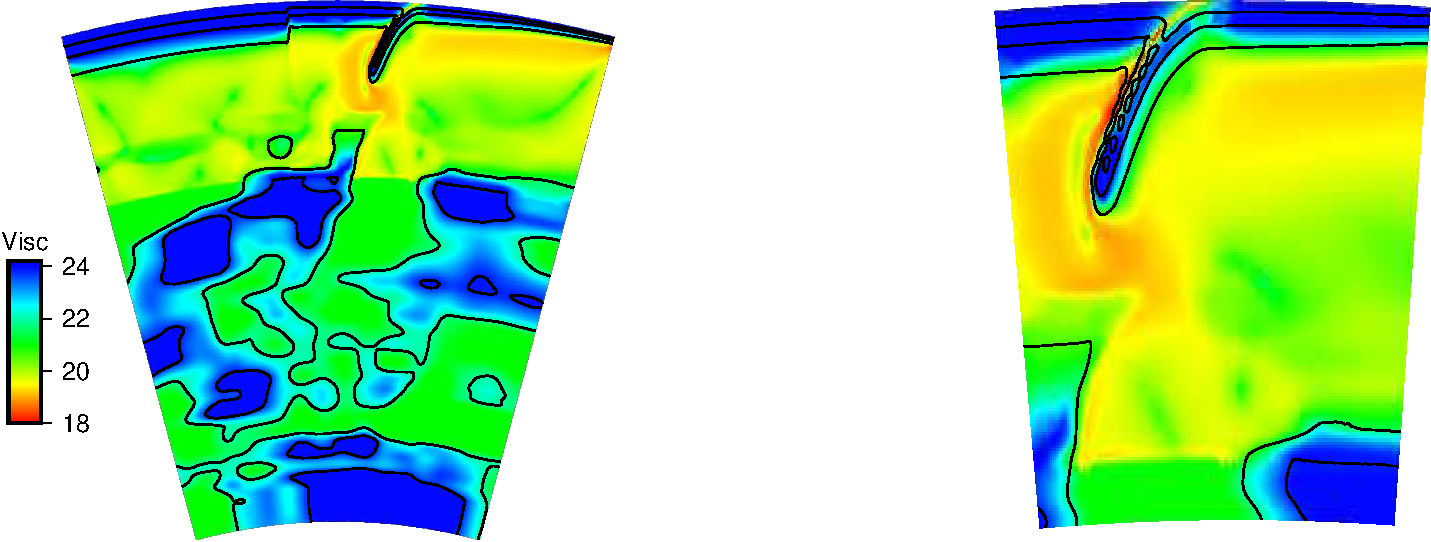
\includegraphics[scale=0.7]{middle.pdf}%{mesh.pdf}
}
%\hspace{-0.2cm}\subfigure[]{
%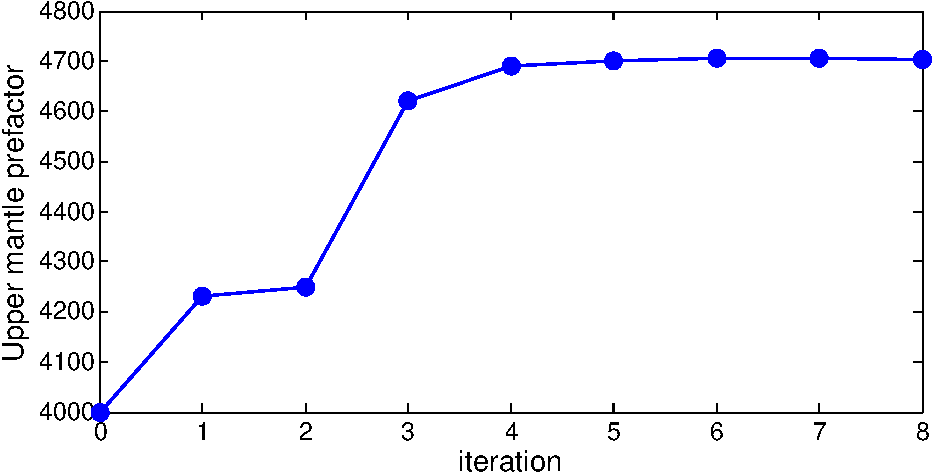
\includegraphics[height=35mm,width=58mm]{um_chap4.pdf}%{mesh.pdf}
%}
\caption{\mgnote{ Case number}
Effective viscosity for (A) Sumatra \mgnote{Need outline of zoom in areas in A and C.} (B) Zoom in of Sumatra subduction zone (C) Central America (B) Zoom in of Central America subduction zone.}
\label{fig:visc_smaller}
\end{figure}

While the larger cross-section (Cases 1-4) has the advantage of having subduction zones of varying seismogenic coupling, it is important to compare the parameter inferences from the larger cross-section (WEP) to other cross-sections with different subduction zones to determine if the global parameters would be of similar magnitude and how. 
The Sumatra subduction zone is of particular interest as it is thought to be one of the more seismically coupled subduction zones. Therefore, we repeat similar case studies as was done for WEP. For Sumatra, we find in Case 21 \mgnote{no Case 21 in Table}, that the global strain rate exponent is 3.08, while 3.063 for when priors are imposed. When it comes to the activation energy, we find a value of $217.4 kJ/mol$ when we do not include prior knowledge, while 
with prior knowledge we find a value of $224.9 kJ/mol$. Furthermore, the inferred yield stress ranges from 132.6 MPa to 141.7 MPa, values that are similar to what were obtained in WEP. While the Sumatra model is a different subuction zone than was was examined in WEP, we find that there is a similar value for the plate coupling for Sumatra.
 % The first case study is shown below in Fig.\ref{fig:inverse1}
\begin{figure}[H]
\centering
%\hspace{-0.2cm}\subfigure[]{
%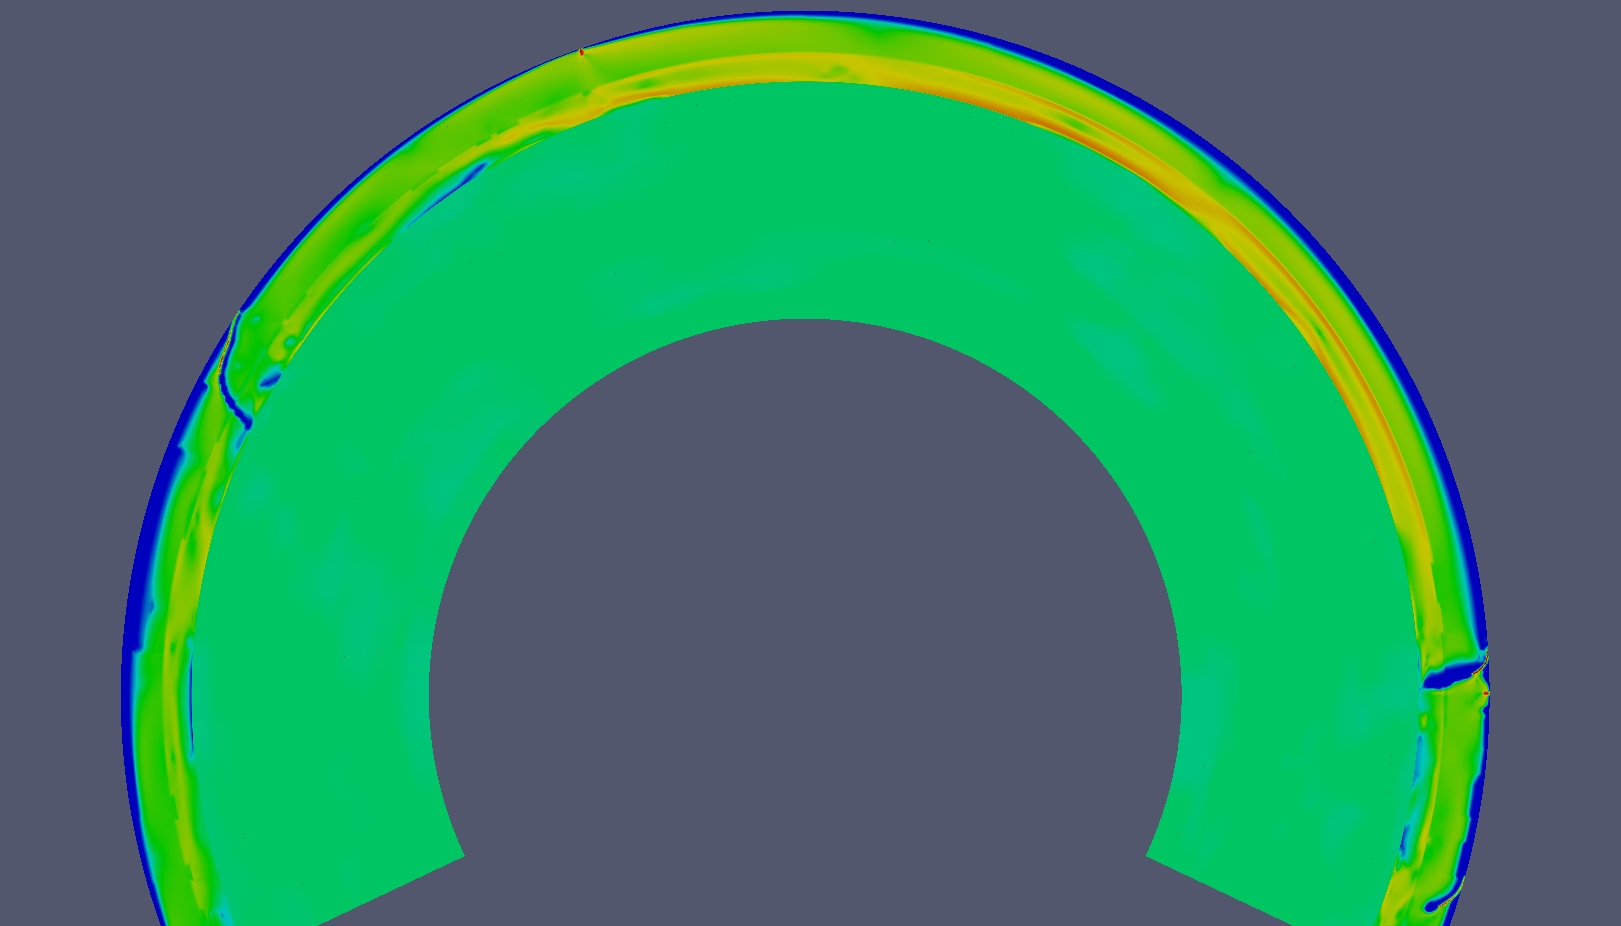
\includegraphics[height=65mm,width=128mm]{visc_no_stress.jpg}%{mesh.pdf}
%}
\hspace{-0.4cm}\subfigure{
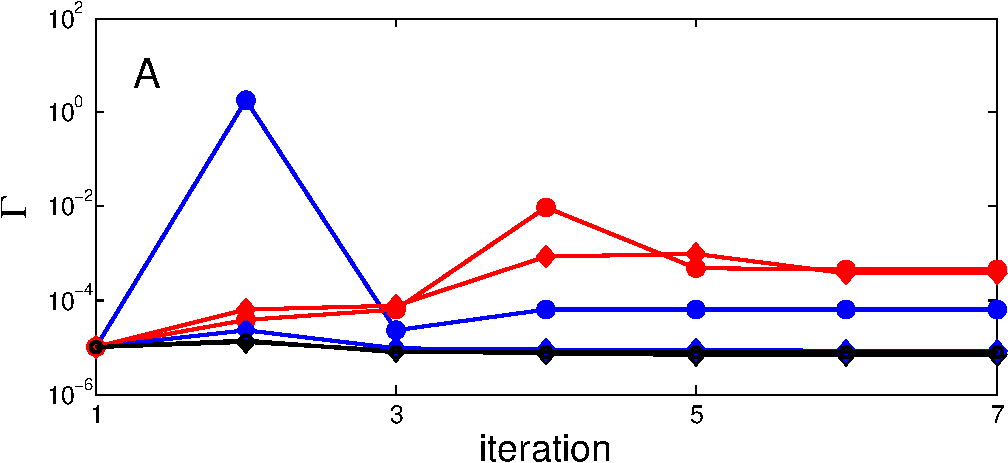
\includegraphics[height=35mm,width=58mm]{fig4a.pdf}%{mesh.pdf}
}
\hspace{-0.1cm}\subfigure{
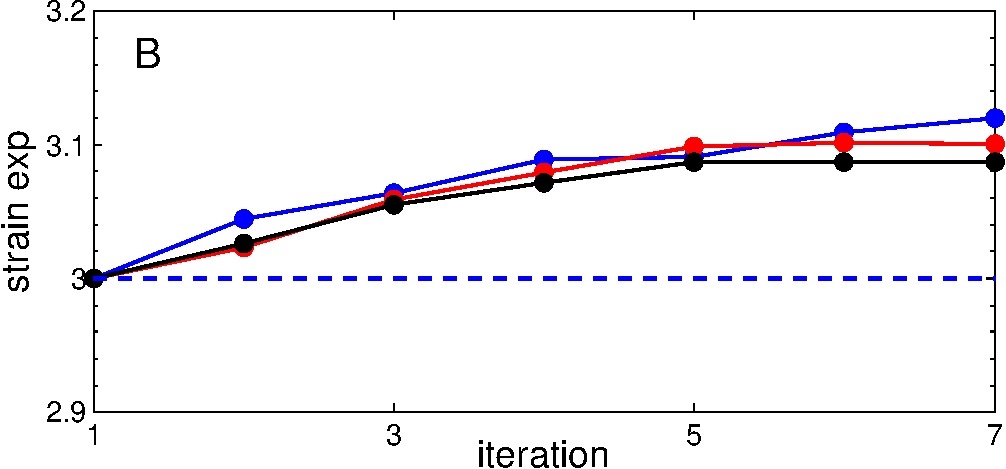
\includegraphics[height=35mm,width=58mm]{fig4b.pdf}%{mesh.pdf}
}
\hspace{-0.2cm}\subfigure{
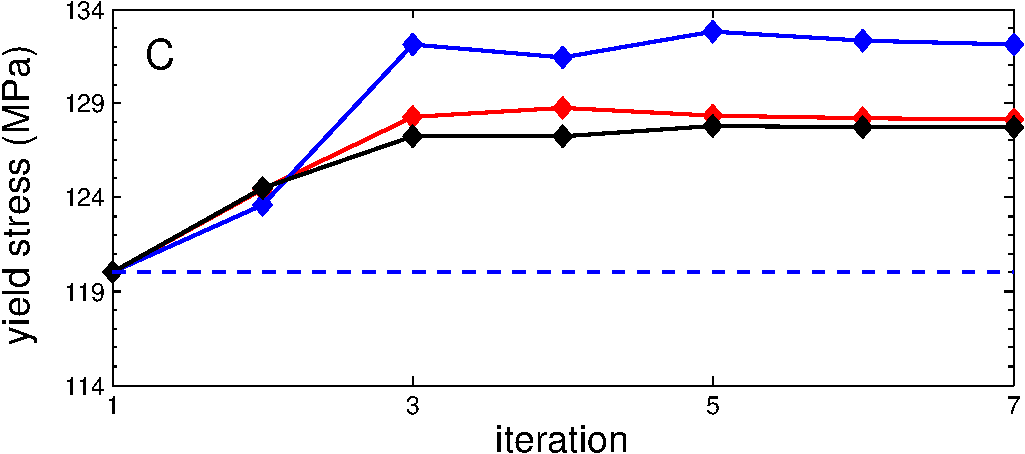
\includegraphics[height=35mm,width=58mm]{fig4c.pdf}%{mesh.pdf}
}
\hspace{-0.2cm}\subfigure{
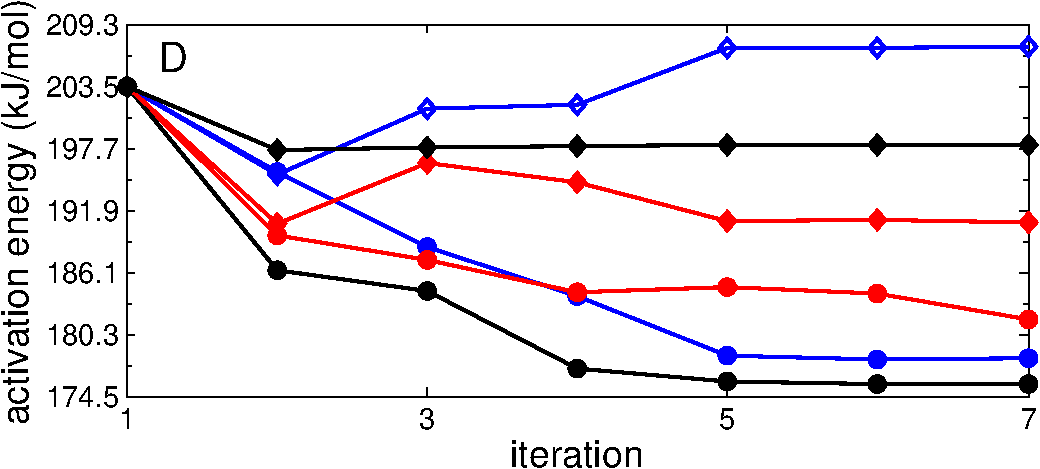
\includegraphics[height=35mm,width=58mm]{fig4d.pdf}%{mesh.pdf}
}
%\hspace{-0.2cm}\subfigure[]{
%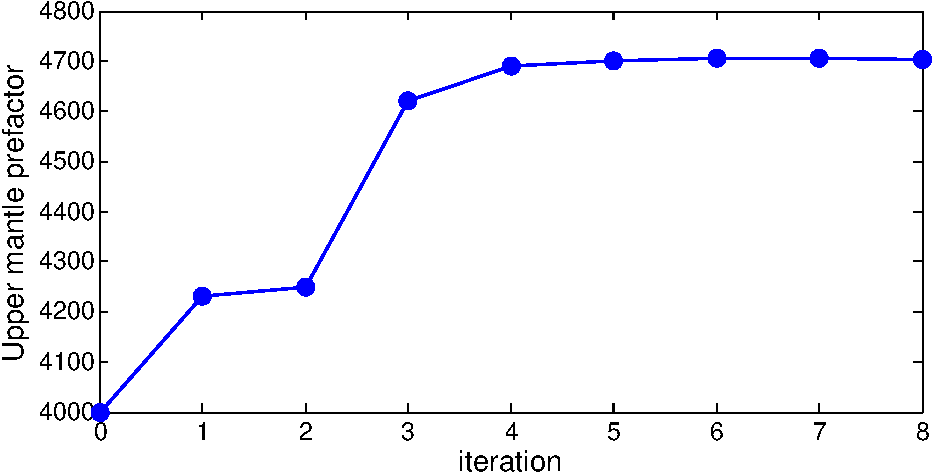
\includegraphics[height=35mm,width=58mm]{um_chap4.pdf}%{mesh.pdf}
%}
\caption{(A) Plate boundary weakfactor iteration for Central America (blue lines), Sumatra (red lines), Tonga (black lines). \textit{Diamonds} \mgnote{Need to use Open Diamond} represent inversion with strain rate exponent held fixed\mgnote{Case ?}, while \textit{circles} represent yield stress held fixed (C) strain rate exponent iteration, \textit{dashed line} represents the fixed value of yield stress (D) yield stress iteration \textit{dashed line} represents the fixed value of the strain rate exponent.
\mgnote{No cap for B? No dashed line in D.}}
\label{fig:inverse1}
\end{figure}
\mgnote{What is the objective here? This \P~ is confusuing because there is all this discussion about Sumatra, but the WEP models are being referred to} We find in Case 5, that the inferred strain rate exponent is approximately 3.05, while the yield stress is approximately 143 MPa. The inferred plate coupling for Sumatra is larger than that of Ryukyu and Izu-Bonin in Cases 1-4, which seems to further suggest that mechanical coupling is independent of rheology. 










\subsection{Uncertainty Quantification for Plate boundary stresses}

An important part of our study is to quantify the uncertainty of the inferred rheological parameters by examining the posterior distributions, specifically the conditional distributions. The conditional distributions convey not only the uncertainty in each parameter, but the trade-offs and how they contribute to the underlying model physics. We compare the conditional distributions for the plate couplings vs. yield stress and strain rate exponent for Case 1  (Fig.\ref{fig:distrib}a,b) and find that there is a clear demarcation between the least coupled subduction zones (Ryukyu and Izu-Bonin) and South America. The partitioning of the subduction zones suggest that the South America plate boundary is more mechanically coupled compared to Ryukyu and Izu-Bonin regardless of the global parameter (yield stress and strain rate exponent). We find a similar partitioning for Cases 2-3 for the larger cross-section and shows that regardless of prior knowledge or addition of average effective viscosity data, there still is a preferential ordering of  plate coupling. 

A consequence of these conditional distributions are the trade-offs between rheological parameters. We see a strong positive correlation between strain rate exponent and yield stress (Fig.~\ref{fig:distrib}c), a negative correlation between the plate couplings and yield stress (Fig.~\ref{fig:distrib}b) and a slight positive correlation between plate couplings and strain rate exponent (Fig.~\ref{fig:distrib}a). The positive correlation between the strain rate exponent and yield stress suggests that as the strain rate exponent increases, plate motions increase, resulting in an increase in yield stress in order to compensate for the increase in plate velocity. 
Yield stress and strain-rate exponent both control the degree of nonlinearity of the system; nonlinearity is increased with larger $n$, so $\sigma_y$ must decrease in order to fit the kinematic constraints.
Likewise, the increase in plate coupling which reduces plate velocity causes an increase in viscosity.  To compensate for this increase in viscosity, a decrease in yield stress is needed, which causes weakening in plates, thereby increasing plate motion. Similarly, as plate coupling increases (increase in viscosity in the fault zone), an increase in the strain rate exponent compensates for the decrease in plate motion.  

\begin{figure}[H]
\centering
\hspace{-0.85cm}\subfigure[]{
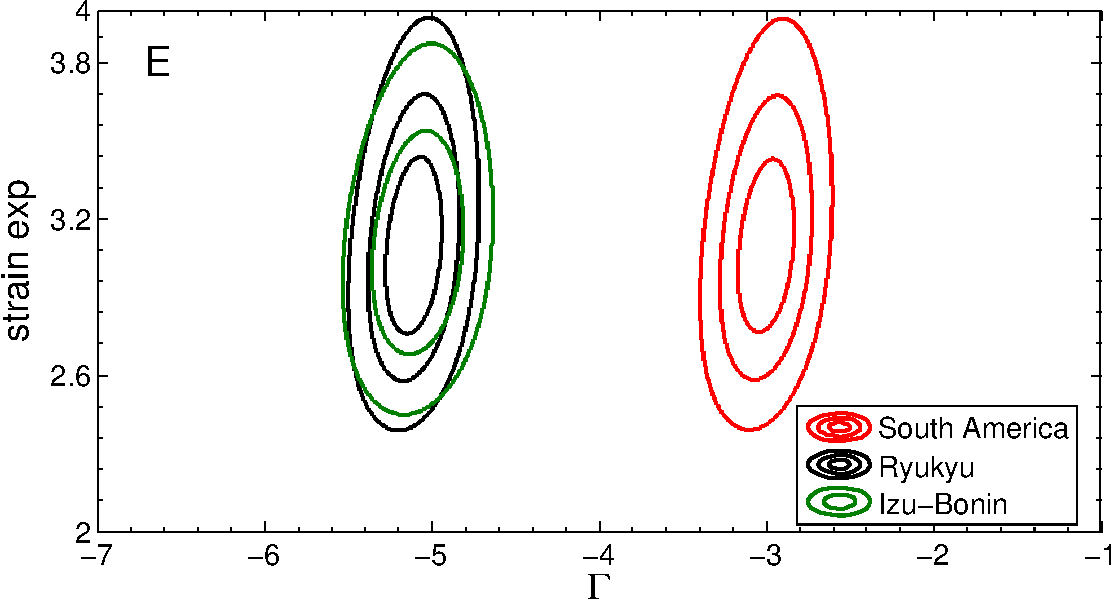
\includegraphics[height=35mm,width=52mm]{fig5a.pdf}%{mesh.pdf}
}
\hspace{-0.1cm}\subfigure[]{
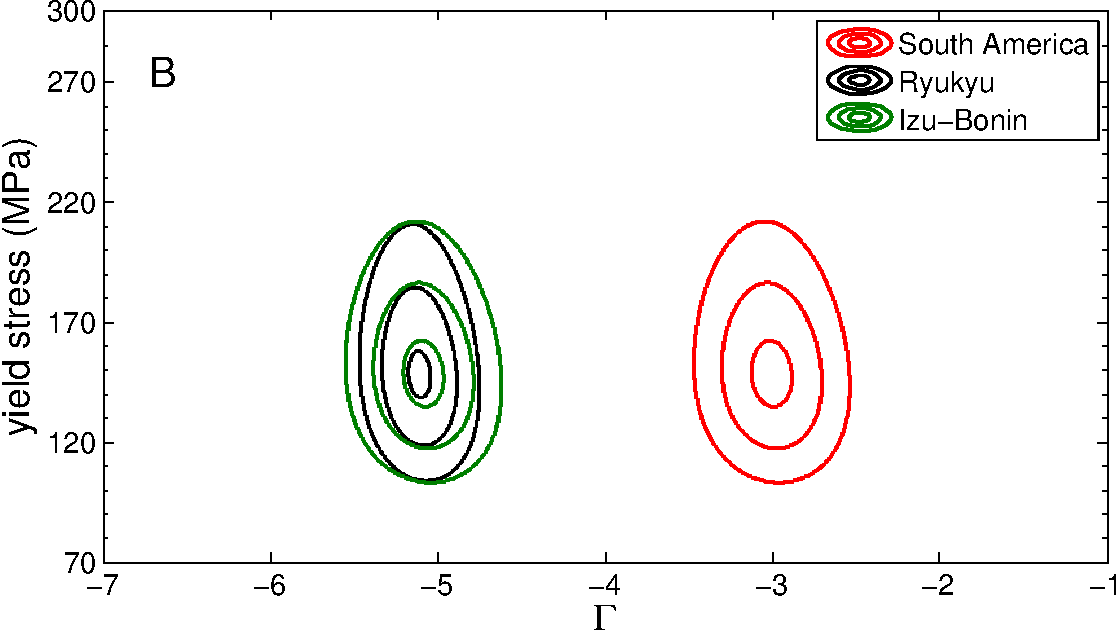
\includegraphics[height=35mm,width=52mm]{fig5b.pdf}%{mesh.pdf}
}
\hspace{-0.1cm}\subfigure[]{
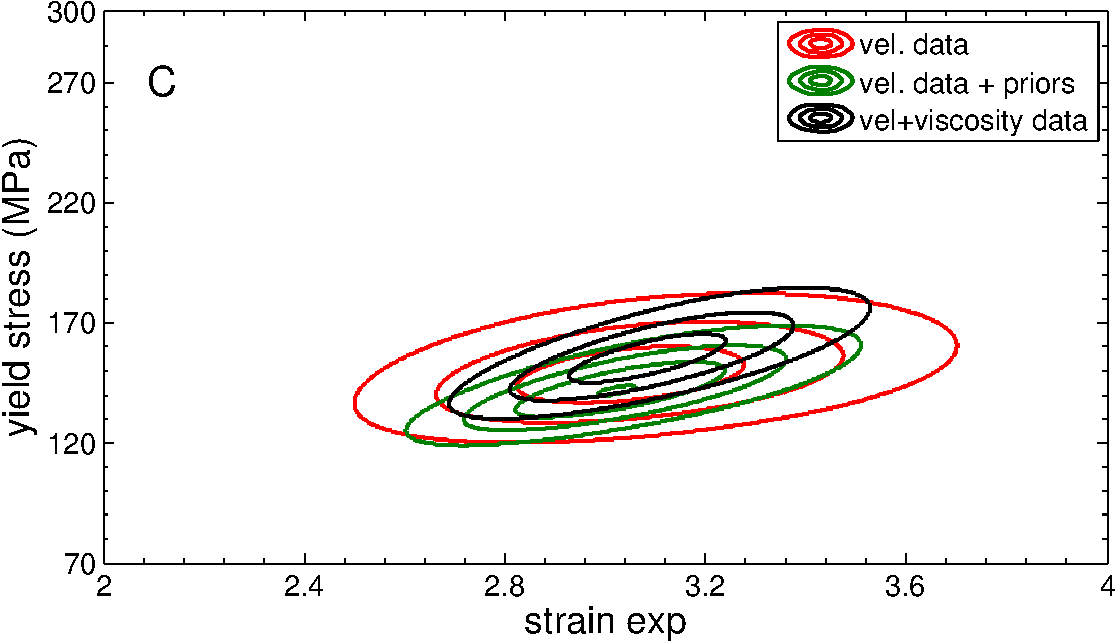
\includegraphics[height=35mm,width=52mm]{fig5c.pdf}%{mesh.pdf}
}
\subfigure[]{
\hspace{-0.8cm}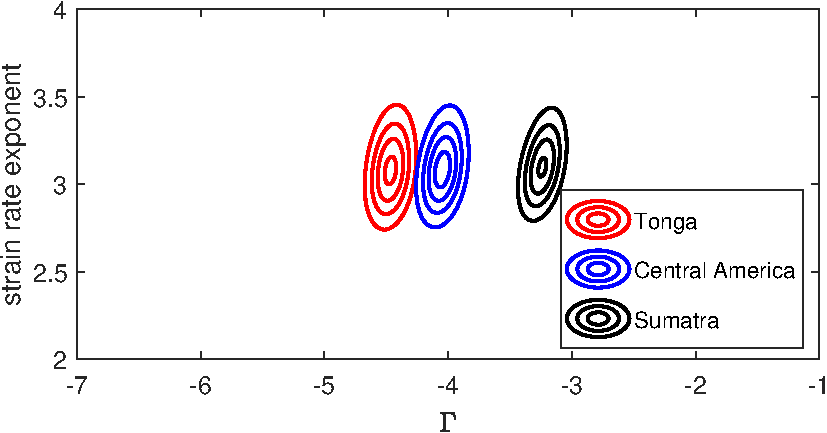
\includegraphics[height=35mm,width=52mm]{fig1new.pdf}%{mesh.pdf}
}
\subfigure[]{
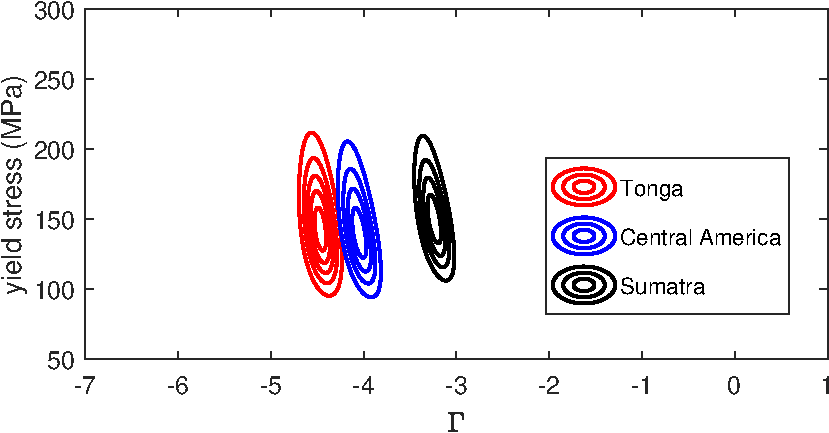
\includegraphics[height=35mm,width=52mm]{fig2new.pdf}%{mesh.pdf}
}
\hspace{0.1cm}\subfigure[]{
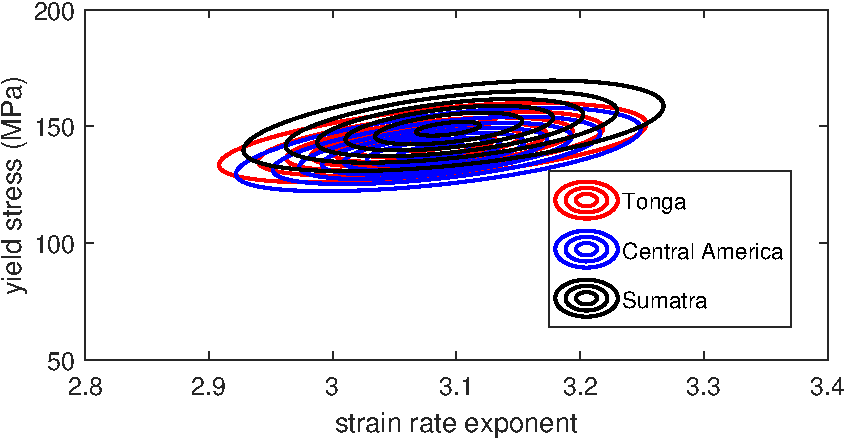
\includegraphics[height=35mm,width=52mm]{fig3new.pdf}%{mesh.pdf}
}
%\hspace{-0.2cm}\subfigure[]{
%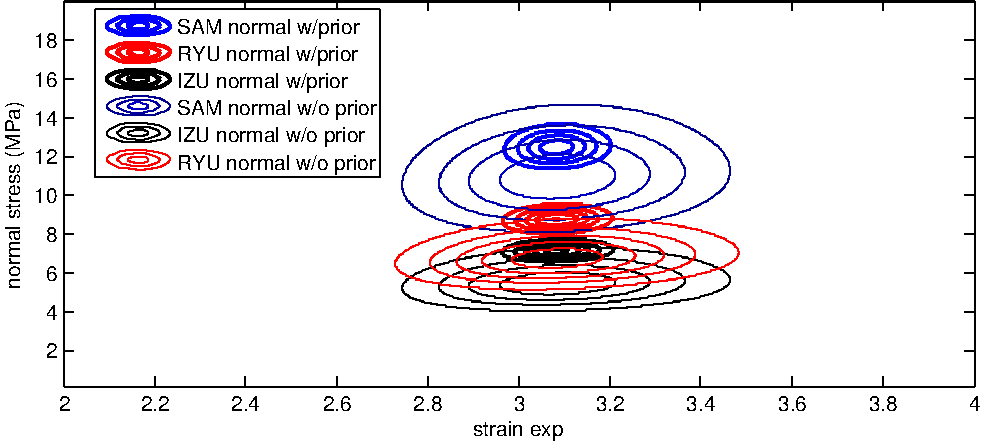
\includegraphics[height=35mm,width=58mm]{normal_comparison_prior2.pdf}%{mesh.pdf}
%}
%\hspace{-0.2cm}\subfigure[]{
%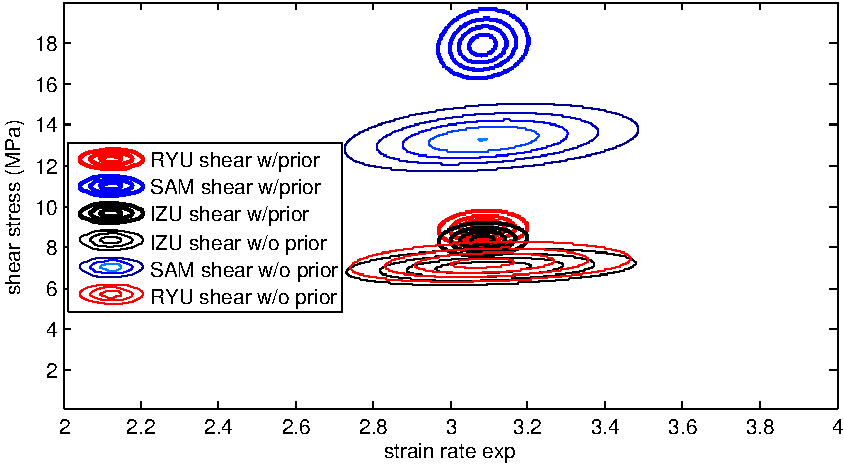
\includegraphics[height=35mm,width=58mm]{shear_comparison_prior.pdf}%{mesh.pdf}
%}
\caption{(A) Strain rate exponent vs. plate coupling. 
(B) Yield stress vs. plate coupling. 
(C) Yield stress vs. strain rate exponent for Case 1 (South America, Ryukyu and Izu-Bonin-(red: velocity constraint, black: velocity + viscosity constraints, blue: velocity constraint + priors) 
(D) Strain rate exponent vs. plate coupling. 
(E) Yield stress vs. plate coupling. 
(F) Yield stress vs. strain rate exponent  (Sumatra (red), Tonga (black) and Central America(blue))
\mgnote{Use fewer contours in the lower panels See me.}}
\label{fig:distrib}
\end{figure}

%An important idea is to know if these trade-offs exist for all inversions, that is with more (or less) inferred parameters, would these correlations remain the same. We find that these trade-offs are consistent when we reduce the parameter space in Case 2, i.e. marginalizing out the upper mantle prefactor, that this there still exists a negative correlation between yield stress and plate coupling in Case 2, which suggests that these rheological parameters are correlated in this way due to the underlying physics with respect to plate motions. Furthermore, we find that there is a positive correlation between the strain rate exponent and yield stress, implying that an increase in strain rate exponent (weakening of the upper mantle) precipitates an increase in yield stress (reduction in plate motion) to make plates resistant to bending.    

An open question about parameter trade-offs deals with additional data, more specifically the average effective viscosity in certain regions of the mantle. 
It is not apparent if these trade-offs will exist with additional data due to the different effects each parameter on both plate motions and average effective viscosity, even though we find similar values for the \textbf{MAP} point between the Case  (without effective viscosity data) and Case 3 (with effective viscosity data). In Fig.\ref{fig:distrib}c we see that the overall distributions are similar in that the trade-offs are the same; however, with the reduction in the variance for the strain rate exponent, the conditional distribution for the strain rate exponent and yield stress, when using average effective viscosity data, is smaller. The additional effective viscosity data acts as prior information marginally reduce the uncertainty on the inferred parameters \mgnote{Is the reduction in the varinces for $\sigma_y$ and $n$ the same?}. 
\mgnote{I think significantly, the slope of the yield stress vs. n increases when the viscosity data is included. Why is this the case? As I asked in the prior section, is the viscosity value that you constrain the system with, larger or smaller than the effective viscosity in the same region without such a constraint. Can you say, that the importance of the yield stress increases when you have added this additional constraint?}

Using prior knowledge can further reduce the variance for the inferred rheological parameters. Using prior knowledge from laboratory experiments \citep{korenaga2008new}, we are able to reduce the variance of the plate couplings and global parameters in Case 4 as shown in Fig.\ref{fig:distrib}c, while retaining the same trade-offs between each rheological parameters, which is expected as we only reduced the acceptable range of the inferred parameters. While the conditional distributions for the larger cross-section show that there is indeed trade-offs in plate couplings and global parameters, is is unknown if these trade-offs exist for all subduction zones. To this end, we compared the conditional distributions for Sumatra, Tonga and Central America (Fig.\ref{fig:distrib}d,e and f). 


In Fig.\ref{fig:distrib}d-e, we find similar trade-offs between the plate coupling and strain rate exponent, that is an increase in plate coupling (an increase in viscosity within the fault zone) would lead to an increase in the strain rate exponent (by promoting more shear thinning) so as to increase plate motion. Similarly, as the plate coupling increases, the yield stress decreases (by promoting more dynamic weakening) so that plates can overcome the resistance from an increase in plate coupling. Furthermore, the same trade-off (positive correlation) between the strain rate exponent and yield stress is found for the Sumatra, Tonga and Central America (Fig.\ref{fig:distrib}f). 

\mgnote{Let's Discuss. Is there a conditional distribution that goes along with this (or these) inversions? Case numbers's?}
We can visually see these trade-offs in the conditional distributions from the effective viscosity in Fig.\ref{fig:visc_smaller} for Sumatra and Central America. We see that there is sufficient \mgnote{Sufficient for what?}strain rate weakening in the upper mantle for each model for both Sumatra and Central America, however, the amount of yielding from dynamic weakening changes in the hinge zone and overriding plate between Sumatra and Central America. \mgnote{Explain more in the proceeding sentance. I think what your saying might be important.}We find in Fig.\ref{fig:visc_smaller} that there is a larger plate coupling for Sumatra relative to Central America, which  yields more dynamic weakening in the overriding plate (more strain). When comparing the effective viscosity of the slabs for Sumatra and Central America, we find that the final viscosity structure suggests that the Central America slab is stronger due to less dynamic weakening and more decoupling between the overriding and subducting plate. \mgnote{Link these arguments to differences in the conditional for these two models}



\begin{figure}[H]
\centering

\hspace{-1.0cm}\subfigure{
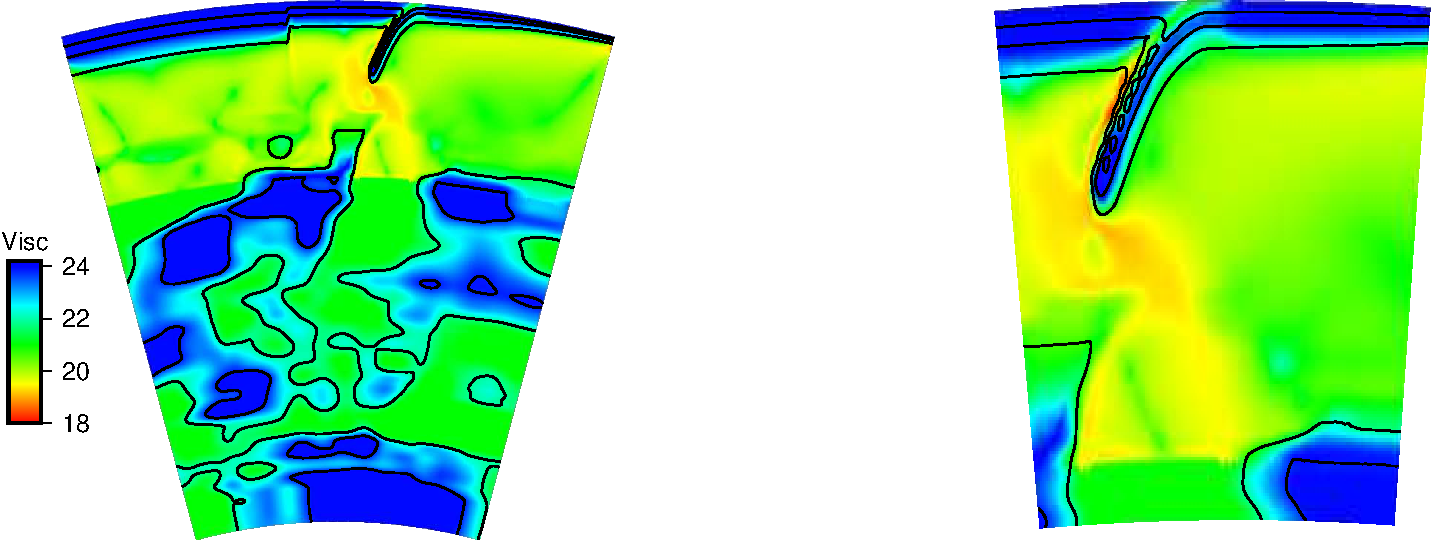
\includegraphics[scale =0.5]{contour_theory.pdf}%{mesh.pdf}
}

\hspace{0.2cm}\subfigure{
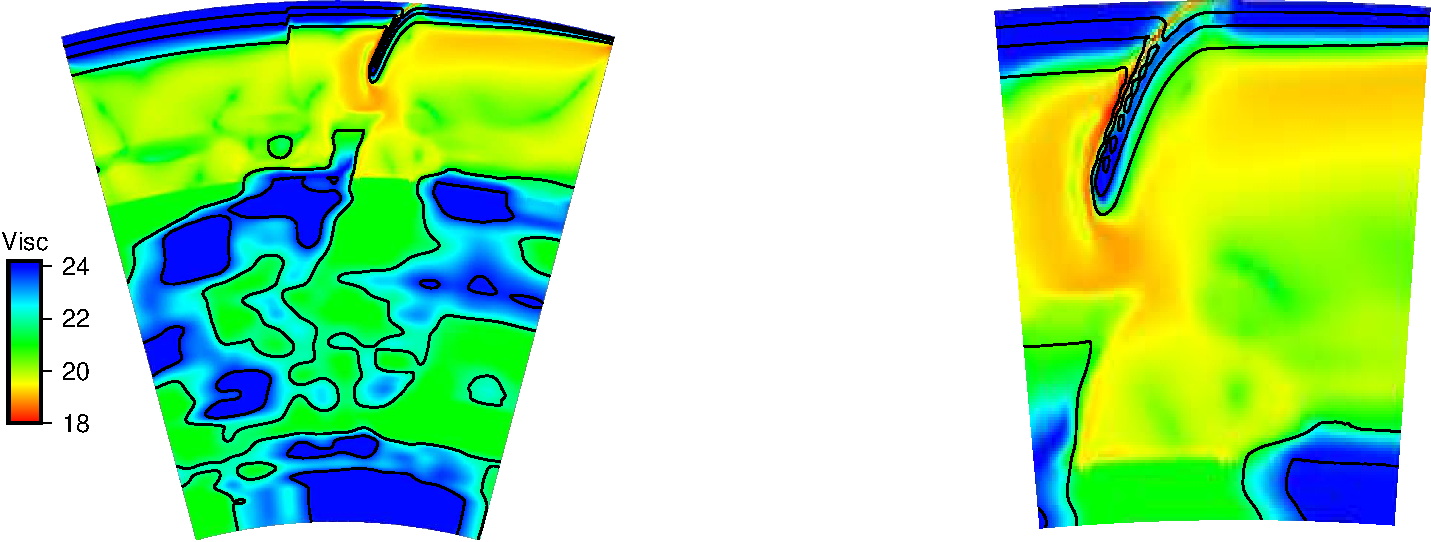
\includegraphics[scale=0.5]{contour_theory2.pdf}%{mesh.pdf}
}
%\hspace{-0.2cm}\subfigure[]{
%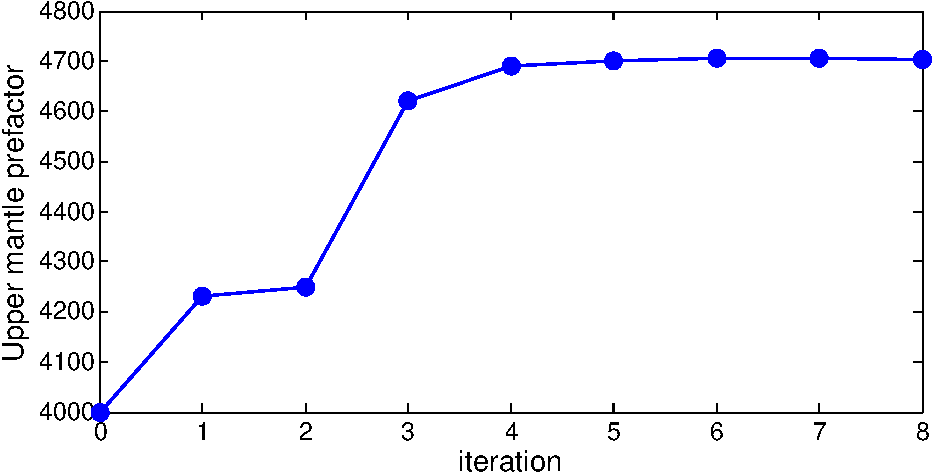
\includegraphics[height=35mm,width=58mm]{um_chap4.pdf}%{mesh.pdf}
%}
\caption{\mgnote{Case numbers's? Are these different iterations for a single inversion} Effective viscosity for a forward model for Middle America (A) Coupled ($\Gamma = 4.0 \cdot 10^{-3}$, $\sigma_y = 160$ MPa, and $n = 3.08$) (B) Zoom in of Middle America and increase in strain rate exponent (C) ($\Gamma = 1.0 \cdot 10^{-5}$, $\sigma_y = 160$ MPa, $n = 3.08$)
(B) Zoom in of Central America subduction zone. \mgnote{You need to consistenly use Middle versus Central America.}}
\label{fig:middle_physics}
\end{figure}

\mgnote{Are these different iterations or different Case numbers's?}To further elucidate these trade-offs, we consider a \mgnote{This is not a thought experiment } thought-experiment where we consider two forward models of Middle America in (Fig.\ref{fig:middle_physics}a). In this example, we consider a coupled Central America subduction zone in Fig.\ref{fig:middle_physics}a, and see  that for a larger coupling the slab would then slow down and the amount of weakening around the slab decreases, resulting in an increase in viscosity around the slab. However, when the coupling is decreased ($\Gamma=4\cdot 10^{-5}$), the amount of strain strain rate weakening increases as does the velocity of the plate. This interplay between the rheological parameters is important as it demonstrates a strong interaction between the global rheological parameters (yield stress and strain rate exponent) and local coupling parameter.



\begin{figure}[H]
\centering
\hspace{-0.85cm}\subfigure{
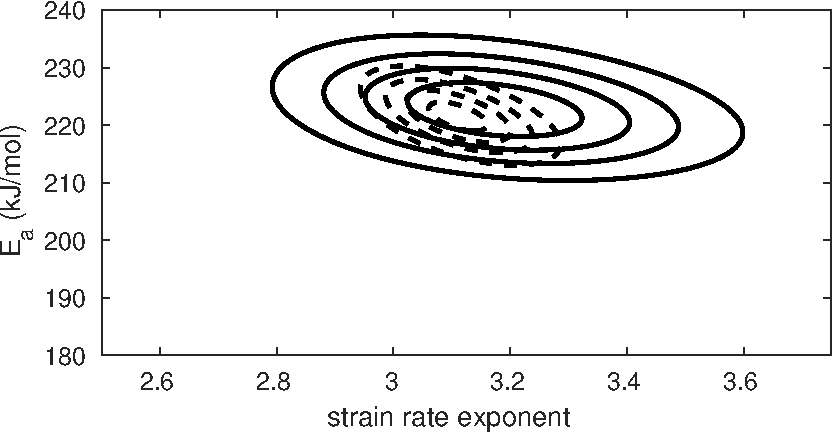
\includegraphics[height=35mm,width=52mm]{ea_strain_large.pdf}%{mesh.pdf}
}
\hspace{-0.1cm}\subfigure{
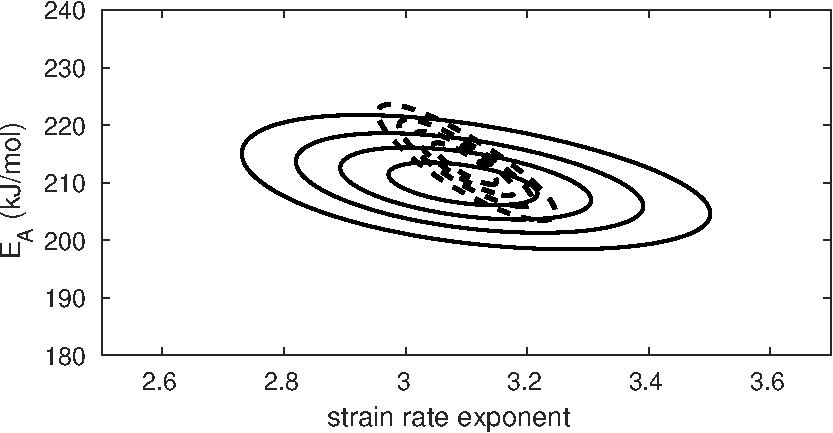
\includegraphics[height=35mm,width=52mm]{ea_strain_sumatra.pdf}%{mesh.pdf}
}
\hspace{-0.1cm}\subfigure{
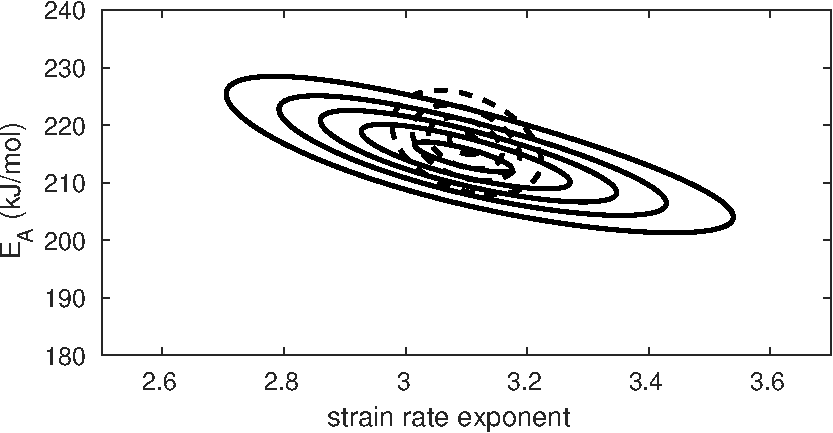
\includegraphics[height=35mm,width=52mm]{ea_strain_central.pdf}%{mesh.pdf}
}
 

\caption{Activation energy vs. strain rate exponent for (A)Sumatra. 
(B) Central America. 
(C) Tonga (Dashed lines include priors)}
\label{fig:activ_distrib}
\end{figure}


One of the key analyses that was developed in this chapter was the characterization of the uncertainty of the stresses (shear and normal) of each plate boundary that is built upon a Gaussian approximation around the \textbf{MAP} point for each inversion. We apply this approach to our models \mgnote{Case numbers}as shown in Fig.\ref{fig:shear_smaller}a,b, where we compare the mean normal and shear stresses of each plate boundary and find that there is a similar pattern of the partitioning between the least coupled subduction zones of Ryukyu and Izu-Bonin to the more coupled subduction zone of South America. Similar to Fig.\ref{fig:distrib}, the same pattern of a more coupled South America plate boundary appears (both normal and shear stresses), regardless of the global parameter. However, we note that the mean of the computed normal stress is lower than the shear stresses, which is certainly not expected.



\begin{figure}[H]
\centering
\hspace{-0.85cm}\subfigure{
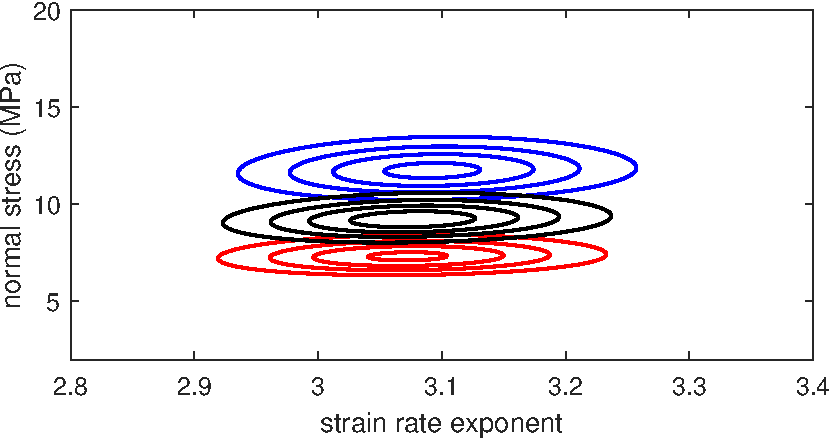
\includegraphics[height=35mm,width=52mm]{fig8new.pdf}%{mesh.pdf}
}
\hspace{-0.1cm}\subfigure{
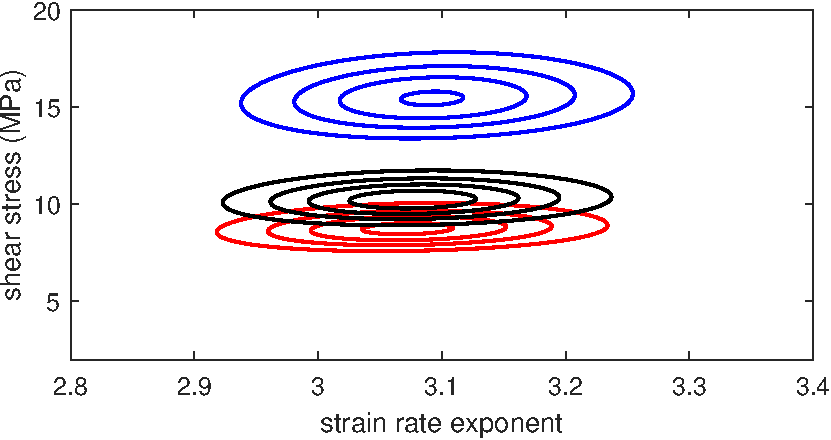
\includegraphics[height=35mm,width=52mm]{fig9new.pdf}%{mesh.pdf}
}

\caption{(A)Normal Stress vs. strain rate exponent. 
(B) Shear stress vs. strain rate exponent. 
 for WEP}
\label{fig:stress_distrib1}
\end{figure}


\begin{figure}[H]
\centering
\hspace{-0.2cm}\subfigure[]{
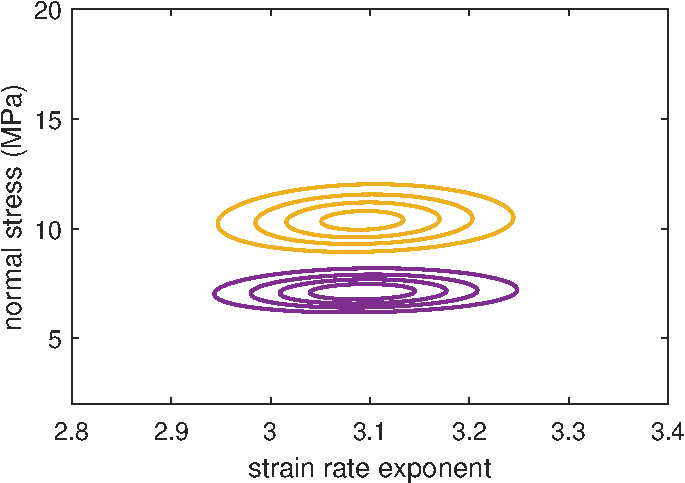
\includegraphics[height=35mm,width=58mm]{fig3.pdf}%{mesh.pdf}
}
\hspace{-0.2cm}\subfigure[]{
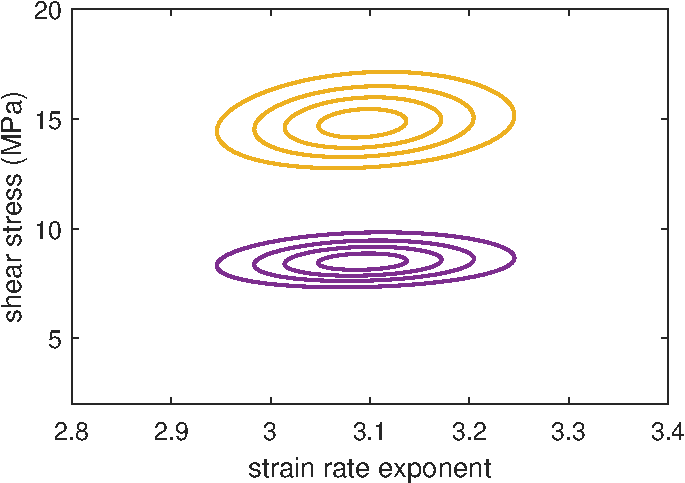
\includegraphics[height=35mm,width=58mm]{fig4.pdf}%{mesh.pdf}
}
\hspace{-0.2cm}\subfigure[normal stresses]{
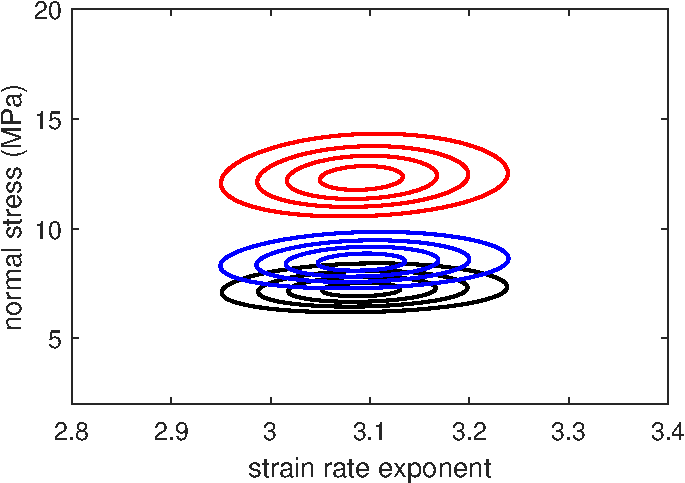
\includegraphics[height=35mm,width=58mm]{fig5.pdf}%{mesh.pdf}
}
\hspace{-0.2cm}\subfigure[shear stresses]{
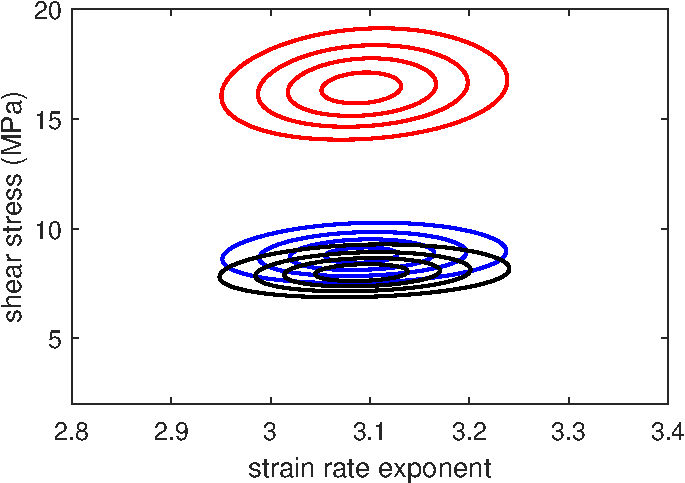
\includegraphics[height=35mm,width=58mm]{fig6.pdf}%{mesh.pdf}
}
\caption{
\mgnote{Need a key}
(A) Normal stress comparison and 
(B) shear stress comparison for Tonga cross section (Yellow contours are for South America while purple contours are for Tonga). 
(C) Normal stress comparison and (D) shear stress comparison for Tonga and South America\mgnote{Different colors are needed in C and D than used in A and B.}}
\label{fig:shear_smaller}
\end{figure}


We similarly compared the stress conditional distributions for Sumatra and Tonga in Fig.\ref{fig:shear_smaller}c,d and find that the shear average shear stress in the fault zones are larger than the normal stress. Similar to South America, we find that there is a partitioning of subudction zones for both shear and normal stresses, where Sumatra is more coupled than Tonga.


\begin{figure}[H]
\centering
\hspace{-0.2cm}\subfigure[]{
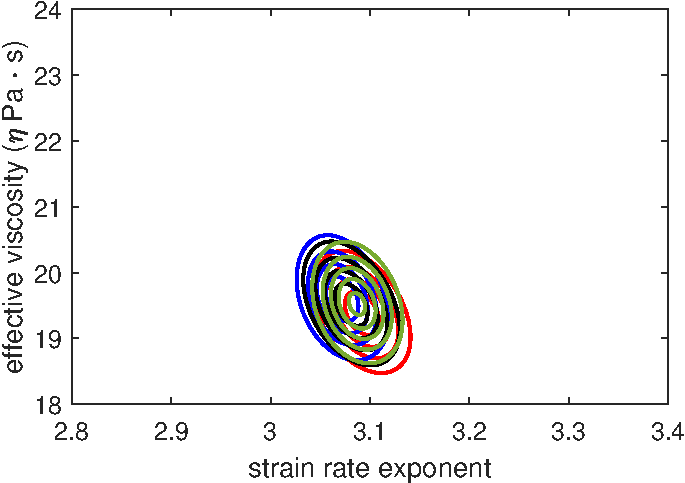
\includegraphics[height=35mm,width=58mm]{fig7.pdf}%{mesh.pdf}
}
\hspace{-0.2cm}\subfigure[]{
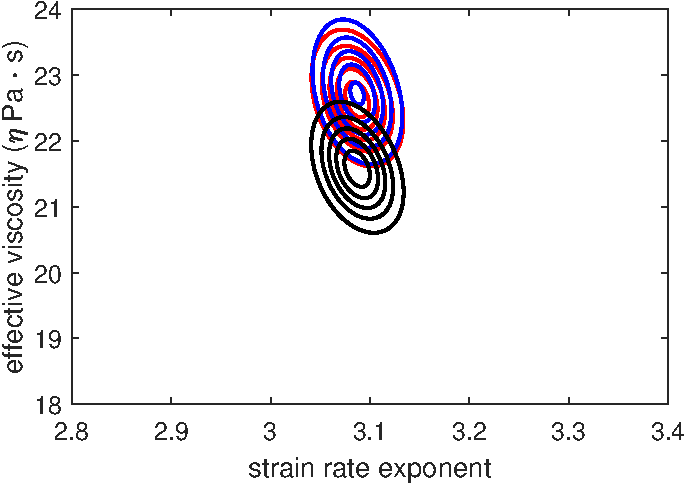
\includegraphics[height=35mm,width=58mm]{fig8.pdf}%{mesh.pdf}
}
\hspace{-0.2cm}\subfigure[normal stresses]{
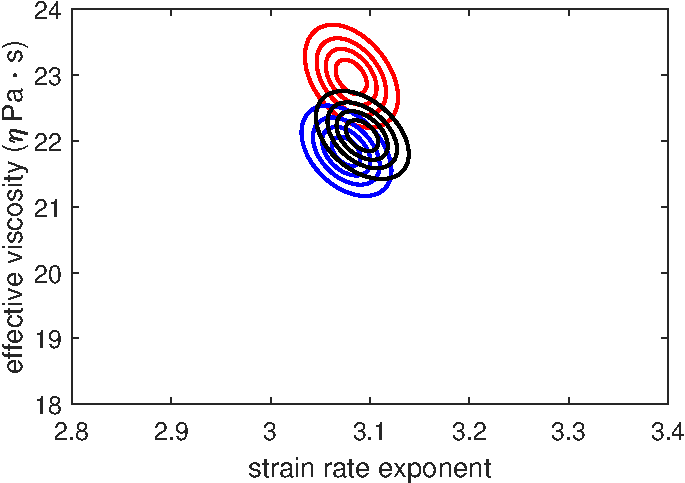
\includegraphics[height=35mm,width=58mm]{fig9.pdf}%{mesh.pdf}
}
\hspace{-0.2cm}\subfigure[shear stresses]{
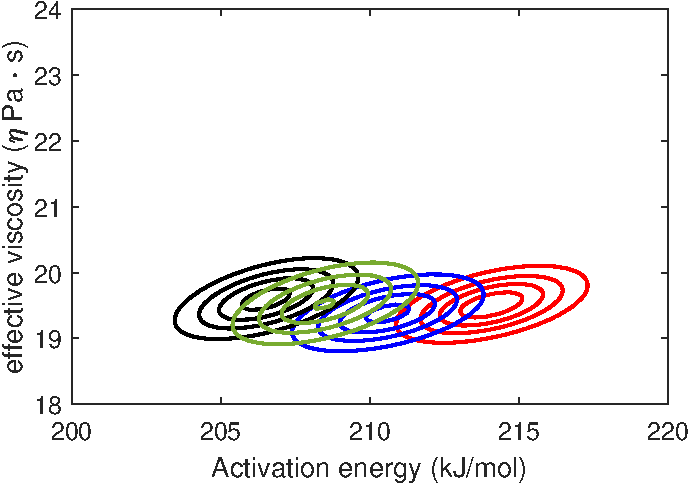
\includegraphics[height=35mm,width=58mm]{fig10.pdf}%{mesh.pdf}
}
\caption{
\mgnote{In A and B there is a 'dashed' line in the label box but no such line in the figures.}
(A) Average Effective Viscosity vs. strain rate exponent in the upper mantle  
(B)  Average Effective Viscosity vs. strain rate exponent in the hinge zones  for Sumatra, Central America and Tonga
(C) \mgnote{where, hinge zone of UM}Average Effective Viscosity vs. strain rate exponent for WEP (D) Average Effective Viscosity vs. Activation energy for WEP, Sumatra, Central America and Tonga}
\label{fig:shear_smaller}
\end{figure}

\section{Discussion}

\mgnote{This section holds considerable promise, but it is very redundant and you need to compare your values to others in the published luterature (cite, compare, discuss)}
Here, we build upon our earlier work \citep{ratnaswamy2015adjoint} including through the addition of effective viscosity data, using realistic temperature and fault zone structures from seismic models, plate motions from a recent kinematic model (MORVEL56), and making estimates of quantities of interest including stresses and average effective viscosities (extrinsic parameters). When incorporating these methods into this optimization framework, we are able to analyze the relationships between the rheological (intrinsic) pparameters vs extrinsic quantities as well as any improvements in the uncertainty we get from adding additional data.
 We considered four crosses sections: (1)WEP (2)Sumatra (3)Tonga and (4) Central America as they represent varying spectrum of the seismic coupling and therefore inferring the rheological parameters for each of these cross-sections can tell us to what degree the inferred parameters vary for each subduction zone. The WEP model contains three subduction zones:(1)South America (2)Izu-Bonin and (3)Ryukyu, where the South America subduction zone is thought to be the most seismically coupled while Izu-Bonin and Ryukyu are thought of as the least seismically coupled \citep{scholz2012seismic}. 

\mgnote{combine all model inferences of n (w/o redundance) before discussing lab experiments} With the WEP model, we found that the strain rate exponent across all models is slightly larger than 3.0 (Cases ). Even without prior knowledge, the likelihood distribution suggests that a \textbf{MAP} point of 3.072 in Case is sufficient to predict observed plate motions. 
  
  The strain rate value of 3.0 is similar with those that obtained from experiments, though those experiments are larger (approximately 3.5). The larger strain rate exponent from from experiments can be due to uncertainty in both the conditions such as pressure and temperature. Furthermore, we find in the Sumatra, Central America and Tonga cases that we infer a strain rate exponent between 3.076-3.12, which is in the range of those obtained in Case for WEP. Therefore, there seems to be a relationship between these 2D models that regardless of the cross-section, the preferred strain rate exponent in the upper mantle should be larger than 3.0. Furthermore, the strain rate we obtain in all of our inversions also show a weak asthenosphere, (approximately $10^{19-20}Pa\cdot s$), which is similarly found in other studies \mgnote{which studies, cite, compare, discuss} that have tried to constrain the average effective viscosity. An important caveat is that while the nonlinear strain rate exponent is important for weakening in the upper mantle, it is not the only physical process as we do not account for water weakening.
  
  The yield stress is an important quantity as it locally controls weakening in the slabs. However, our yield stress is not simply comparable to Byerlee law since is is not depth-dependent. We typically find yield stresses that are approximately $150 \space MPa$ in our inferences for the WEP cross-section. While the 150 MPa value is global for this cross-section it does not have the same effect for each subduction zone, that is there is a different amount of dynamic weakening in each of the slabs. We find in Fig., that there is more dynamic weakening in the hinge zone for the Nazca plate compared to Ryukyu and the Pacific plate. This dynamic weakening is a product of both the plate coupling and the yield stress. We note that this yield stress is larger than those from estimates in seismicity, as it is assumed that the yield stress should be less than $10 \space MPa$. However, by the very nature our models only can inform how strong slabs because we do not allow for yielding in the fault zones.
  
  Therefore, a large yield stress value such as $132 MPa$ suggests that slabs are sufficiently strong \mgnote{defer slab strength issue until you considewr the effective viscosity (since three parameters give rise to slabs strength)} such that they can accommodate large stress values which is not a surprise as it has been thought that slabs are strong enough to be stress guides \citep{Stadler27082010}. In Case , the yield stress of 150 MPa suggests that slabs need to not only have a larger viscosity contrast but need to have a certain stress threshold to propagate stresses from the mantle to the plates. An important question is how large of a viscosity contrast relates to the stresses within slabs. Within our forward models, we apriori bound the effective viscosity by $\mathcal{O}(10^6)$, where the majority of the viscosity variations occur between the slab and the weak-zone. Therefore, the relationship between the effective viscosity and stress within slabs is best understood from the point of view of the viscosity variations between the asthenosphere and slab. In our models, the average effective viscosity within the slab is approximately $10^{24}\space Pa\cdot s$, while the average effective viscosity in the asthenosphere is $3\cdot 10^{20}\space Pa\cdot s$, or approximately $\mathcal{O}(10^4)$ in viscosity variations. Therefore, there seems to be a minimum value of variations in viscosity for slabs to act as stress guides \mgnote{I didn't understand your argument, let's discuss}.   

\mgnote{It seems to me that th eyield stress is notvarying strongly between the X-sectional models.}
We also find that there is a variation in the dynamic weakening for Sumatra, Central America and Tonga subduction zones. While the inferred yield stresses for each of those models vary between 135-147 MPa, they still exhibit different amounts of weakening in the hinge zone, where there is more of a reduction of the effective viscosity for Sumatra compared to Tonga and Central America.
  
  The activation energy is an important quantity that we added to our parameter inferences for each of the cross-sections. We find that the inferred activation energy is approximately 215 kJ/mol for the WEP cross-section in Case . Similarly, we note that in the smaller cross-sections in Sumatra, that the activation energy is 219 kJ/mol. We find that this value provides sufficiently strong plates and slabs while providing a strong contrast between the effective viscosity of the upper mantle and the plates. As mentioned earlier, there is a relationship between the amount of dynamic weakening in the hinge zone based on the amount of coupling and the yield stress. \mgnote{Move the rest of the paragraph and combine with seismic coupling}Looking at the WEP cross-section, we find that for all the cases () there is a partitioning of the weakfactors for each subduction zone. In each case, we find that there is at least an order of magnitude of increase in the South America subduction zone weakfactor compared to Ryukyu and Izu-Bonin. Furthermore, the weakfactor for Ryukyu is similar to Izu-Bonin, with Ryukyu's weakfactor being slightly larger than Izu-Bonin. Furthermore, we find that with this increased weakfactor for South America, there is more dynamic weakening in the more coupled South America subduction zone so as to 
  
  An important recurring result within our inversions is the trade-offs between the rheological parameters such as the strain rate exponent and yield stress. To review, the weakfactor controls the amount of resistance along the plate-boundary  interface, the strain rate exponent controls the amount of shear-thinning, while the yield stress controls the amount of weakening within plates and slabs. In each of the cross-sections (WEP, Sumatra, Tonga and Central America) we find that there is a negative correlation between the strain rate exponent and the yield stress, evident in generic models \citep{ratnaswamy2015adjoint}. This result is significant as it suggests that the even with the MORVEL56-NNR plate motion model, there still is a preferred correlation between the strain rate exponent and yield stress. Further examining the negative correlation between the strain rate exponent and yield stress, when there is significant yielding in hinge zone as in WEP (Fig.)\mgnote{I don't follow this}, the reduction effective viscosity causes the slab to fall into the upper mantle, which increases the strain rate and effectively increases plate speed due to the reduced bending force. Therefore, to compensate for this increase in plate motion either the strain rate exponent or weakfactor must change.
  
  The correlation between the weakfactor and yield stress is an emergent trade-off we see within all the cross-section models. We find that as the weakfactor increases (channel in the fault zone becomes more viscous), there is a negative correlation between the yield stress. This negative correlation implies that when the weakfactor increases, there is a reduction in the yield stress which promotes weakening in the hinge zone to counter the increased resistance. In particular, we see that as yielding occurs as plates bend in the Nazca plate in WEP, we find that the weakfactor is comparably larger than Ryukyu and Izu-Bonin (where both of those subduction zones have less yielding). Similarly, this trade-off occurs in the Sumatra model, where we see that there is a significant amount of coupling while there is sufficient yielding within the slab. This trade-off between the weakfactor and yield stress comes about because the increased resistance from the plate coupling causes more weakening around the slab to allow for it to fall into the upper mantle.  The Middle America cross-section represents the opposite case compared to Sumatra, that is, there is a decoupling between the overriding plate and subduction zone. This decoupling represents an increase in plate speeed, therefore to compensate for the increase in plate velocity would require an increase in the bending force in the hinge zone-that is there would be an increase in the yield stress to increase the bending force.
  
There seems to be a correlation between the intrinsic mechanical coupling (weakfactor) and the seismic coupling in Table \ref{table:parameters} \mgnote{correct Table}. Notably, there is a delineation of subduction zones between those that are mechanically coupled. In all of our WEP models, we find that the South America subduction zone is the most (mechanically) coupled compared to Ryukyu regardless of which parameter we held fixed. The other end of the spectrum is where there is the relationship between the mechanical coupling and seismic coupling. We find that for the Sumatra cross-section, there is a larger mechanical coupling than Central America.
   
   \begin{table}[H]
  \caption{Summary of seismic coupling coefficients ($\chi_s$) is the seismic coupling coefficient, while $\chi_g$ is the geodetic coupling coefficient \citep{scholz2012seismic}.} % title of Table
  \centering  % used for centering table
  \begin{tabular}{c c c c c c} % centered columns (2 columns)
    \hline \hline                        %inserts double horizontal lines
    Subduction Zone & $\chi_s$ & $\chi_g$ & $\sigma_n (MPa)$ & $\sigma_t (MPa)$ & $\Gamma$ \\ [0.5ex] % inserts table
    %heading
    \hline                  % inserts single horizontal line
    Izu-Bonin &0.01 &N/A &7.22 &7.99 & $7.42 \cdot 10^{-6}$\\
    South Ryukyu  &0.05 &N/A &8.47&8.72 & $9.11 \cdot 10^{-6}$\\
    Central Chile &0.70 &1.0 &12.3 &16.4 & $7.02 \cdot 10^{-4}$ \\
    Sumatra &0.5-0.83 &1.0 &11.73 & 15.33 &$3.93 \cdot 10^{-4}$\\
    Central America &0.10 &0.20 &9.22 & 10.23 & $5.51 \cdot 10^{-5}$ \\
    North$/$South Tonga & $0.66/0.14$ &N/A &7.32 & 8.74 & $8.32 \cdot 10^{-5}$ \\
    \hline %inserts single line
  \end{tabular}
  \label{table:coupling_summary} % is used to refer this table in the text
\end{table}

   
   While we are able to estimate the mechanical coupling between subduction zones, we need to look at the stresses within the subduction zones to compare to those provided by seismological constraints. We find that in all our cases (WEP, Sumatra, Central America and Tonga) that the estimates of shear and normal stresses are less than 20 MPa, which satisfies seismological constraints\mgnote{constraints, Cite, compare, discuss}, suggesting that the inferred rheological parameters give rise a reasonable state of stress. While the stress values are in the correct range, we find that the conditional distributions have bounds on how large the stresses are-which are under 20 MPa. Examining the stress conditionals for WEP, we find that the \textbf{MAP} point for the shear stresses are consistently larger than those of the normal stresses. 
Many models of subduction with a frictional material have a shear stress that is a fraction of the normal stress.
Here, we have purely viscous flow, Couette flow in a low viscosity  channel, adjacent o the  moving slab.
   
   Ultimately, these \textbf{MAP} point values are within range of values that are acceptable; however, we need to take into account these viscous stress values are related to seismic couplings. A subduction zone that is very coupled has a seismic coupling close to 1.0., while those that are least seismically coupled have values closer to 0.  In Table \ref{table:parameters}, we see that the seismic and geodetic coupling ($\chi_s$ and $\chi_g$) for Peru (Central and South), while Chile and Sumatra have larger geodetic couplings that are large, while Tonga has a seismic coupling that is less than 1 in Table \ref{table:parameters}. We find a similar ordering compared to that obtained from seismic coupling, in that the largest shear stresses belong to the South America, Sumatra plate boundaries compared to Izu-Bonin, Ryukyu and Tonga-which suggests that there is a correlation between mechanical and seismic coupling. However, 3D models are needed to truly test if these relationships. Furthermore, extensions of this work should seek to include plasticity within the fault zones for a better estimate of the shear and normal stresses there; however, with plasticity included, there are additional parameters such as the cohesion that needs to be accounted for. In these studies, we have laid the foundation for using multiple pieces of data to better constrain the strain rate exponent. Furthermore, we extended our formulation to forward predict the uncertainty in the extrinsic quantities by generating a Gaussian approximation to the shear and normal stresses. Those approximations for the stresses show that there is a partitioning of seismically coupled subduction zones in the mechanical sense, which suggests that regardless of what the strain rate exponent and  yield stress, there is a preferred mechanical coupling of subduction zones. To verify this result, it needs to be tested out with global models.
                 








\appendix
\section{Derived Covariance Estimates}
We have previously set models in how to estimate quantities that are are inferred such as the stresses. In this section, we will thoroughly discuss how to apply this Gaussian approximation to various quantities of interest. Mapping of covariance matrices from one space to another requires  a transformation,i.e. using the Jacobian. As an example, we will look at transforming a Gaussian distribution for the inferred yield stress and strain rate exponent, that is $\ppi(\mm):= \mathcal{N}([n,\ssigma_y],\mathcal C) \rightarrow \ssigma(\gamma \mm)$, where we look at the scaled space between the parameters. To determine the mapping of the covariance we make use of,
\underline{Case 1: 1D Normal}
\begin{equation}
\frac{\partial \ssigma}{\partial \mm} = \gamma
\end{equation}
leading to
\begin{equation}
\ppi_2 = \mathcal N(\mu,\gamma^2\sigma)
\end{equation}
\underline{Case 2: 2D Normal}
We consider the case when we apply a stretch factor in the form of $\gamma = [\gamma_1, \gamma_2]$, that is $\mm = [\mm_1, \mm_2]$. Therefore $\ssigma = [\gamma_1 \mm_1, \gamma_2 \mm_2]$. The follwoing now holds
\begin{equation}
\frac{\partial \ssigma}{\partial \mm} = 
\begin{bmatrix}
\gamma_1 & 0 \\
0 & \gamma_2 \\
\end{bmatrix}
\end{equation}
leading to
\begin{equation}
\mathcal C = 
\begin{bmatrix}
\gamma_1^2 a & \gamma_1 \gamma_2 b \\
\gamma_1 \gamma_2 b & \gamma_2^2 c \\
\end{bmatrix}
\end{equation}

\begin{equation}
\ppi_2 = \mathcal N(\mu,\gamma^2\sigma)
\end{equation}
An important point is to construct the covariance matrix for the relationship between the stress and inferred parameters (strain rate exponent, yield stress). To do so, we form the vector $\ssigma_{a}$ such that  $\ssigma_a = (\ssigma, n,\sigma_y..)^\intercal$. Doing so, we find the Jacobian is
\begin{equation}
\frac{\partial \ssigma_a}{\partial \mm} = \frac{\partial [\ssigma, n, \sigma_y...]^\intercal}{\partial \mm}
\end{equation}
which results in 
\begin{equation}
\mathcal C = 
\begin{bmatrix}
\frac{\partial \ssigma}{\partial n} & \frac{\partial \ssigma_{a}}{\partial \sigma_y} \\
\frac{\partial n}{\partial n}& \frac{\partial n}{\partial \sigma_y} \\
\frac{\partial \sigma_y}{\partial n}& \frac{\partial \sigma_y}{\partial \sigma_y} \\
\end{bmatrix}
\end{equation}
which leads to 
\begin{equation}
\mathcal C = 
\begin{bmatrix}
\frac{\partial \ssigma}{\partial n} & \frac{\partial \ssigma_{a}}{\partial \sigma_y} \\
1 & 0\\
0 & 1 \\
\end{bmatrix}
\end{equation}

\begin{figure}[H]
\centering
\hspace{-1.2cm}\subfigure{
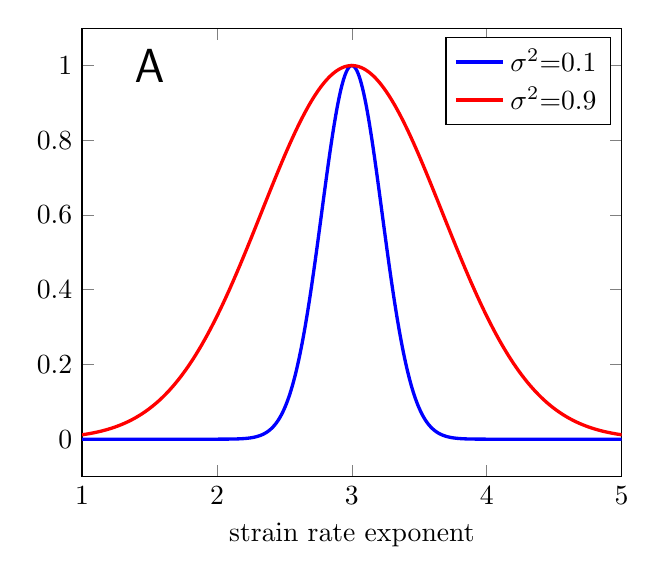
\begin{tikzpicture} 
\begin{axis}[ xlabel=strain rate exponent,xmin=1.0, xmax=5.0 ] % invoke external gnuplot as % calculator: 
  \addplot [mark=none,very thick, blue, samples=1000]{exp(-(x-3.0)^2/0.1)}; 
  \addlegendentry{$\sigma^2$=0.1}
  \addplot [mark=none,very thick, red, samples=1000]{exp(-(x-3.0)^2/0.9)}; 
  \addlegendentry{$\sigma^2$=0.9}
\node[font=\fontsize{18}{18}\sffamily] at (axis cs:1.5,1.0){A};


\end{axis} 
\end{tikzpicture}
}
\end{figure}
\subsection*{Uncertainty estimates for Effective viscosity}
While we have developed this machinery for normal and shear stresses, we can extend it to the effective viscosity in a region. The average effective effective viscosity we are interested in is,
\begin{equation}
 \eta_{avg} = \exp(\int_{\Omega_i} \log \eta d\Omega_i)
 \end{equation}
The jacobian is then,
\begin{equation}
\frac{\partial \eta_{avg}}{\partial \mm} = \eta_{avg}\int_{\Omega_i} \frac{\eta){,i}}{\eta}
\end{equation}
The transformation then yields 
\begin{equation}
\mathcal C = 
\begin{bmatrix}
\frac{\partial \ssigma}{\partial n} & \dots & \frac{\partial \ssigma_{a}}{\partial \sigma_y} \\
1 &  0 & \dots & 0\\
0 & 1 & \dots & 0 \\
\vdots & \vdots & \ddots  & 0 \\
0 &0 & \dots & 1 

\end{bmatrix}
\end{equation}
%\section*{Conclusion}

\bibliography{references}


\end{document}
